\NeedsTeXFormat{LaTeX2e}[2005/12/01]
%%    2010/04/06 v1.0 Vorlage Master-Forschungspraktikum Versuchsauswertung
%%    based on the 2009/10/14 v0.1 GAUBM template by Prof Pruschke

\documentclass[twoside,        %% zweiseitiges Layout
               BCOR12mm,       %% Bindekorrektur 12 mm
% please comment out if report is in English
               english,ngerman, %% Dokumentspr. Deutsch, Alternativspr. Englisch
% please remove comment if report is in English 
%               ngerman,english, %% Dokumentspr. Englisch, Alternativspr. Deutsch
               fleqn,headsepline=false,footsepline=false
              ]{Vorlage/MFPREPORT}
\makeatletter
\DeclareOldFontCommand{\rm}{\normalfont\rmfamily}{\mathrm}
\DeclareOldFontCommand{\sf}{\normalfont\sffamily}{\mathsf}
\DeclareOldFontCommand{\tt}{\normalfont\ttfamily}{\mathtt}
\DeclareOldFontCommand{\bf}{\normalfont\bfseries}{\mathbf}
\DeclareOldFontCommand{\it}{\normalfont\itshape}{\mathit}
\DeclareOldFontCommand{\sl}{\normalfont\slshape}{\@nomath\sl}
\DeclareOldFontCommand{\sc}{\normalfont\scshape}{\@nomath\sc}
\makeatother

%% Pakete und Definitionen ausgelagert
\usepackage{a4}
\usepackage{multicol}

% language option set in JGNSUM class
\usepackage{babel}
\usepackage{hyperref}

%% FONT:
%\usepackage{lmodern}
\usepackage{times} % sieht besser aus als lmodern
%\usepackage{palatino} % sieht schlechter aus als times
%\usepackage{mathpazo} % very ugly font, to be loaded later ???
%\usepackage{cmbright} % doesn't work either
\usepackage[T1]{fontenc}
\usepackage{textcomp}

\usepackage{ucs}
\usepackage[utf8x]{inputenc}

\usepackage{amsfonts}
\usepackage{amstext}
\usepackage{amsmath}
\usepackage{amsthm}
\usepackage{amssymb}
\usepackage{amsbsy}   % AMS-Boldsymbol

% \usepackage{mathabx} % e.g. for \Sun
%% but not a standard package (neither texlive nor Miktex)
%% so use wasysym (\astrosun) instead
\usepackage{wasysym} % e.g. for \astrosun or \CheckedBox

\usepackage{bbm,mathrsfs}

\usepackage{textcomp} % noch einige coole symbole

\usepackage{sectsty}
\allsectionsfont{\raggedright}

\usepackage[numbers]{natbib}
\citestyle{dinat}
\bibliographystyle{dinat}

\usepackage{makeidx}

\usepackage{url}	% für hübsche URLs mit Link
\usepackage{color}	% für farben a la \definecolor{Gray}{gray}{0.5}
\usepackage{verbatim}
\usepackage{subfigure}
\usepackage{listings}

\usepackage{fancybox}
%usage:
%\begin{Verbatim}[frame=single,label=Titel]
%Verbatim Zeile
%\end{Verbatim}


 \setlength{\textwidth}{16.2cm}
 \setlength{\textheight}{24cm}
 \setlength{\oddsidemargin}{0cm}
 \setlength{\evensidemargin}{-0.5cm}

 %unbedingt nach abmessungen einfügen!
 \usepackage{fancyhdr}
 \pagestyle{fancy}
 %\sloppy % für weniger absatzfehler

 \setcounter{tocdepth}{2}
 \setcounter{secnumdepth}{2}

 \ifreportelse{\numberwithin{equation}{chapter}}{\numberwithin{equation}{section}}
 \theoremstyle{plain}% default
 \ifreportelse{\newtheorem{thm}{Theorem}[chapter]}{\newtheorem{thm}{Theorem}[section]}

 \newtheorem{satz}{Satz}
 \newtheorem{lem}[thm]{Lemma}
 \newtheorem{prop}[thm]{Proposition}
 \newtheorem{kor}[thm]{Korollar}
 \newtheorem{cor}[thm]{Corollary}

 \theoremstyle{definition}
 \newtheorem{defi}{Definition}

 \def\@proof{%
  \if@englishpreamble{Proof}\else{Beweis}\fi
 }
 \newenvironment{bew}{\begin{proof}[\@proof]}{\end{proof}}



%% einbinden einiger nützlicher Befehle
\newcommand{\iflanggerman}[2]{
 \iflanguage{german}{#1}{
  \iflanguage{ngerman}{#1}{#2}
 }
}

% box around the whole equation, number inclusive
\newcommand{\boxedeqn}[1]{%
  \[\fbox{%
      \addtolength{\linewidth}{-2\fboxsep}%
      \addtolength{\linewidth}{-2\fboxrule}%
      \begin{minipage}{\linewidth}%
      \begin{equation}#1\end{equation}%
      \end{minipage}%
    }\]%
}

\iflanggerman{
 \newcommand{\const}{\mathrm{konst}}
 \newcommand{\Const}{\mathrm{konst.}}
}{
 \newcommand{\const}{\mathrm{const}}
 \newcommand{\Const}{\mathrm{const.}}
}

% von Meier
\newcommand{\nbd}{\nobreakdash-\hspace{0pt}}
% example: $K$\nbd{}Vektorraum
\newcommand*{\transpose}[1]{\prescript{t}{}{#1}}
\newcommand*{\conjugate}[1]{\overline{#1}}
\newcommand*{\abs}[1]{\lvert#1\rvert}
\newcommand*{\Mod}{\mathrm{mod}}
\newcommand{\symdif}{\mathbin\triangle}
\DeclareMathOperator{\Graph}{Graph}
\DeclareMathOperator{\id}{id}
\DeclareMathOperator*{\grad}{grad}
\DeclareMathOperator*{\Div}{div}
\DeclareMathOperator*{\rot}{rot}
\DeclareMathOperator{\sig}{sig}
\DeclareMathOperator{\sgn}{sgn}
\DeclareMathOperator{\diag}{diag}
\DeclareMathOperator{\tr}{tr}
\DeclareMathOperator{\Sp}{Sp}
\DeclareMathOperator{\im}{Im}
\DeclareMathOperator{\re}{Re}

\newcommand{\vcentcolon}{\mathop{:}}



%Zur Formatierung in der Matheumgebung
\renewcommand{\t}{\ensuremath{\rm\tiny}} % Tiefgestellter Text in der Matheumgebung wird schoener mit: $\Phi_{\t{Text}}$
\renewcommand{\d}{\ensuremath{\mathrm{d}}} % Die totale Ableitung ist stets aufrecht zu setzen: \d
\newcommand{\diff}[3][]{\ensuremath{\frac{\d^{#1}#2}{\d#3^{#1}}}} % einfache Ableitung nach x: $\ddx{\Phi}$
\newcommand{\pdiff}[3][]{\ensuremath{\frac{\partial^{#1}#2}{\partial#3^{#1}}}} % wie gesprochen, eine partielle Ableitung: \del
\newcommand{\aeqiv}{\ensuremath{\qquad \Longleftrightarrow \qquad}} % Eine Aequivalenz
\newcommand{\folgt}{\ensuremath{\qquad \Longrightarrow \qquad}} % Ein Folgepfeil mit Abstaenden
\newcommand{\corresponds}{\ensuremath{\mathrel{\widehat{=}}}} % Befehl für "Entspricht"-Zeichen
\newcommand{\mi}[1]{\ensuremath{\mathit{#1}}} % italics für griechische Buchstaben in Matheumgebung

%Um nicht so viel schreiben zu müssen...
\newcommand{\bs}[1]{\boldsymbol{#1}}
\newcommand{\ol}[1]{\overline{#1}}
\newcommand{\wtilde}[1]{\widetilde{#1}}
\newcommand{\mrm}[1]{\mathrm{#1}}
\newcommand{\mbf}[1]{\mathbf{#1}}
\newcommand{\mbb}[1]{\mathbb{#1}}
\newcommand{\mcal}[1]{\mathcal{#1}}
\newcommand{\mfrak}[1]{\mathfrak{#1}}

%Abkürzungen
\newcommand{\zB}{z.\,B.\ }
\newcommand{\bzw}{b.\,z.\, w.\ }
\newcommand{\Dh}{d.\,h.\ }
\newcommand{\Gl}{Gl.\ }
\newcommand{\Abb}{Abb.\ }
\newcommand{\Tab}{Tab.\ }

\usepackage{cleveref}
\usepackage{braket}


\begin{document}
\LabratoryName{FM.ULP}{Spatial and Temporal Distortion of Ultrashort Light Pulses}
\ProtocolAuthor{Eric}{Bertok}{eric.bertok@stud.uni-goettingen.de}
\Assistant{Dr. Sabine}{Steil}
\ResearchFocus{Festkörper- und Materialphysik (M.phy.403)}
% In der naechsten Version beruecksichtigt
%\Collaborator{Vorname}{Nachname}{email}
\ConductedOn{22}{11}{2017}
\date{\today}
% eines von beiden
\CopyNotWanted
%\CopyWanted

\pagenumbering{roman}
\maketitle

%\begin{otherlanguage}{english}
%\end{otherlanguage}

\tableofcontents

\clearpage
\pagenumbering{arabic}

\section{Einleitung}
\label{sec:einleitung}
In dem Bereich der Optik wurden in den letzten Jahren Laser entwickelt, die in
der Lage sind, Pulse zu erzeugen, welche nur einige Femtosekunden lang sind. Da
man für die Messung von kurzen Phänomenen einen physikalischen Prozess
benötigt, der noch kürzer ist, hat diese Erfindung einen Einblick in viele
dynamische Prozesse auf der Femtosekundenskala. Ein Beispiel ist der Bereich
der Femtochemie.
Da Ultrakurze Pulse aufgrund der Unschärferelation aus sehr vielen Frequenzen
bestehen, sind sie besonders von Dispersion betroffen. Es treten eine Vielzahl
von zeitlichen, aber auch räumlichen Dispersionen und Verzerrungen auf, die
exemplarisch in diesem Versuch sowohl qualitativ als auch quantitativ
untersucht werden. 
Es wird ein GRENOUILLE Pulscharakterisierungsgerät verwendet, um diese
Verzerrungen wie räumliche und zeitliche Dispersion, Chirp und den Pulse-Front
Tilt zu messen. Dabei kommen verschiedene optische Bauteile zum Einsatz, um
deren Einfluss auf den Puls zu untersuchen. Ein Prismenkompressor wird
verwendet, um die Verzerrungen mit theoretischen Erwartungen zu vergleichen.
\section{Theorie}
\label{sec:theorie}
\subsection{Grundlagen}
Zur Beschreibung Ultrakurzer Laserpulse verwendet man einen semiklassischen
Ansatz, bei dem die Maxwell-Gleichungen für eine makroskopische Polarisation
gelöst wird. Im Folgenden wird das Vektorfeld des elektrischen Feldes $\vec E$
durch einen Skalar $E$ genähert \cite{Diels2006}. Hiermit wird eine für das Experiment
relevante Polarisationsrichtung beachtet. Im Allgemeinen sind auch Effekte
möglich, bei denen verschiedene Polarisationsrichtungen miteinander koppeln,
was eine genauere Betrachtung erfordert.
Ausgehend von dem elektrischen Feld $E(t)$ definiert man mithilfe der Fouriertransformation das komplexe Spektrum
$\tilde{E}(\omega)=\mathcal{F}[E(t)]=\int_\mathbb{R}E(t)e^{-i\omega t}\d t
\label{eq:FT}$.
Die Rücktransformation ergibt sich zu $E(t)=\mathcal{F}^{-1}[\tilde
E(\omega)]=\frac{1}{2\pi}\int_{\mathbb R}\tilde E(\omega)e^{i\omega t}\d
\omega$. Dies funktioniert aufgrund der Linearität der Maxwell Gleichungen. Die
Lösung kann somit in eine Superposition von ebenen Wellen zerlegt werden. Hier
ist $\omega$ die Kreisfrequenz der ebenen Welle. Nach Konvention wird häufig
nur der positive Anteil des Spektrums betrachtet. Er hat aufgrund der
Reellwertigkeit von $E$ den vollen Informationsgehalt \cite{Diels2006}
. Bei der Fourier-Rücktransformation integriert man so nur über alle
positiven $\omega$.
Ein Puls wird nun beschrieben durch \cite{trebinolec}
\begin{align}
    E(t)=\frac{1}{2}\sqrt{I(t)}\exp\left(i\left[ \omega _0 t-\Phi(t)
    \right]\right),
    \label{eq:efield}
\end{align}
wobei $\omega_0$ die sog. Trägerfrequenz und $\phi(t)$ eine allgemeine Phase in
Abhängigkeit von der Zeit $t$ ist. Die Trägerfrequenz ist der oszillatorische
Anteil des Pulses innerhalb der Einhüllenden $\sqrt{I(t)}$ und wird häufig in
eine komplexe Einhüllende $E_0$ integriert. Die Phase $\phi(t)$ beschreibt die
Zeitliche Veränderung der Farbe des Pulses. $I(t)=|E(t)|^2$ ist die
Intensität des Pulses. Ist $I$ eine stark gepeakte Funktion, so redet man von
einem ``ultrakurzen Puls''. Analog kann man durch $S=|\tilde E(\omega)|^2$ die
spektrale Intensität einführen. Somit gilt $\tilde
E(\omega)=\sqrt{S(\omega)}\exp(-i\varphi(\omega))\label{eq:spectrum}$, wobei
$\varphi(\omega)$ die spektrale Phase ist. Diese ist zentrale Größe bei der 
Beschreibung von gechirpten Pulsen (siehe unten).
Die Beschreibung des Spektrums ist auch mithilfe der Wellenlänge $\lambda$
möglich. Die Umrechnung ergibt sich zu \cite{trebinolec}:
\begin{align}
    S_\lambda(\lambda)=S_\omega\left(\frac{2\pi c}{\lambda^2}\right)\frac{2\pi
    c}{\lambda^2}.
    \label{eq:lambdaspec}
\end{align}


\subsection{Instantane Frequenz und Chirp}
Die instantane Frequenz eines ultrakurzen Pulses ist definiert als
\cite{trebinolec} 
\begin{align}
    \omega_{\text{inst}}=\omega_0-\diff{\phi}{t},
    \label{eq:instfrequ}
\end{align}
mit der Phase $\phi$ und der Trägerfrequenz $\omega_0$. Man kann nun sowohl die Phase, als auch die spektrale Phase taylorentwickeln: 
\begin{align}
    \phi(t)&=\phi_0+\underbrace{\diff{\phi}{t}|_{t=0}}_{\phi_1}t+\underbrace{\diff[2]{\phi}{t}|_{t=0}}_{\phi_2}\frac{t^2}{2}+\cdots,\\
    \varphi(w)&=\varphi_0+\underbrace{\diff{\varphi}{\omega}|_{\omega=\omega_0}}_{\varphi_1}(\omega-\omega_0)+\underbrace{\diff[2]{\varphi}{\omega}|_{\omega=\omega_0}}_{\varphi_2}\frac{(\omega-\omega_0)^2}{2}+\cdots.
    \label{eq:taylor}
\end{align}
Hier ist $\varphi_1=\diff{\varphi}{\omega}|_{\omega=\omega_0}$ der sogenannte
``group delay''(GD) und
$\varphi_2=\diff[2]{\varphi}{\omega}|_{\omega=\omega_0}$ die ``group delay
dispersion (GDD). Hieraus ist zu sehen: Ein nicht verschwindendes $\phi_1$
erzeugt nach \cref{eq:instfrequ} einen konstanten Offset in der instantanen
Frequenz. Dies resultiert nach dem Fourier shift theorem \cite{Diels2006} in einer
Verschiebung im Spektrum. Andersherum erzeugt ein nicht verschwindender GD
einen Offset in der temporalen Intensität. Dies ist zur Bestimmung von
Pulslängen irrelevant. Ist jedoch $\varphi_2$ ungleich Null, so kommt es zur
Dispersion: Die Gruppengeschwindigkeit ändert sich für verschiedene Frequenzen
unterschiedlich und der Puls verläuft. Einen solchen Puls nennt man (linear) gechirpt. Analoges passiert bei einem nicht verschwindenden $\phi_2$. Die instantane Frequenz ändert sich hier linear mit der Zeit.

\subsection{Gaußpuls und Bandprodukt}
\label{seq:bandprod}
Die am einfachsten zu handhabende Pulsform ist die eines Gaußpulses:
\cite{Diels2006} 
\begin{align}
    E(t)=E_0\exp\left[-2\ln 2\left(\frac{t}{\tau_{\text{FWHM}}}\right)\right].
    \label{eq:gaus}
\end{align}
$\tau_{\text{FWHM}}$ bezeichnet die ``full-width half maximum'', also die Halbwertsbreite des Pulses, welche eine von vielen Definitionen zur Beschreibung der Puls- oder Spektralbreite ist. Sie ist definiert als die Breite an der halben Pulshöhe. Im Folgenden wird stets $\tau\equiv\tau_{\text{FWHM}}$ gesetzt. Der Gaußpuls ist neben seiner einfachen Handhabbarkeit auch eine der am häufigsten auftretenden Pulsformen.\\
Da (Kreis-) Frequenz und Zeit konjugierte Variablen einer Fourier
Transformation sind, gilt für sie die Unschärferelation, genannt
``Zeit-Bandbreite-Produkt'': \cite{Diels2006} 
\begin{align}
    \braket{\omega^{2}}\braket{t^{2}} \geq \frac{M^{4}}{4}\kappa_c,
    \label{eq:time-bandwidth}
\end{align}
wobei $\braket{\Delta\omega^{2}}$ bzw $\braket{\Delta t^{2}}$ die Pulsbreite
bzw die Bandbreite -berechnet durch das zweite Moment- bezeichnet. $M$ ist ein
Formfaktor, der die Abweichung zum idealen Gaußpuls bezeichnet \cite{Diels2006}. $\kappa_c$ ist der Chirpfaktor, welcher angibt, dass bei gechirpten Pulsen das Zeit-Bandbreiteprodukt größer ist, als für ungechirpte Pulse. Einen ungechirpten Puls bezeichnet man demnach auch als ``Fourier-limitiert''. Fourier-limitierte Pulse sind also für eine konstante Bandbreite stets am kürzesten.
Die Umrechnung von den zweiten Momenten zur Halbwertsbreite ist für Gaußpulse
einfach über die Varianz einer Gaußverteilung zu berechnen. Es gilt
$\tau=2\sqrt{2 \ln 2}\braket{t^2}$. Aus \cref{eq:time-bandwidth} mit $M=1$ und
$\kappa_c=1$ lässt sich ebenfalls $\braket{\omega^2}=\frac{1}{4 \braket{t^2}}$
durch die Halbwertsbreite ausdrücken. Ausgedrückt durch die reguläre Frequenz
$\nu$
erhält man
\begin{align}
    \label{eq:bandprodeasy}
    \Delta \nu \Delta t = 0.441.
\end{align}

\subsection{Dispersion im Medium}
Bewegt sich ein Lichtpuls durch ein Medium, so wird eine Transferfunktion im
Frequenzraum zum elektrischen Feld multipliziert \cite{trebinolec}: $\tilde
E_{\text{out}}(\omega)=\tilde{E}_{\text{in}}(\omega)\exp(-\alpha(\omega)L)\exp(-i
n(\omega)k_0L)$. Hier beschreibt $\alpha$ die Absorption, welche in diesem
Versuch ignoriert wird. $n(\omega)$ ist der Brechungsindex des Materials in
Abhängigkeit von der Frequenz, $k_0$ ist die Wellenzahl bei der Trägerfrequenz
und $L$ ist die Länge des Materials. Relevant für die Verbreiterung von
Pulslängen ist die Modulation der spektralen Phase. Aufgrund der Form der
Transferfunktion wird diese direkt hinzuaddiert \cite{trebinolec}:
\begin{align}
    \varphi_{\text{out}}(\omega)=\varphi_{\text{in}}+n(\omega)k_0L.
    \label{eq:transferphase}
\end{align}
Eine Taylornäherung des Wellenvektors $k(\omega)=n(\omega)k_0$ ergibt analog zu
\cref{eq:taylor} die sog. ``group velocity dispersion'' (GVD): \cite{trebinolec} 
\begin{align}
    \text{GVD}=k''(\omega_0)=\frac{1}{2}\frac{\lambda_0^3}{2\pi c_0^2}\diff[2]{n}{\lambda},
    \label{eq:gvd}
\end{align}
mit der Trägerwellenlänge $\lambda_0$ und der Lichtgeschwindigkeit $c_0$.
Es gilt GDD $=$ GVD $ L$.
Der wellenlängenabhängige Brechungsindex berechnet sich aus der Sellmeier
Gleichung \cite{refr}:
\begin{align}
    n^2(\lambda)=\frac{B_1 \lambda^2}{\lambda^2-C_1}+\frac{B_2 \lambda^2}{\lambda^2-C_2}+\frac{B_3 \lambda^2}{\lambda^2-C_3},
    \label{eq:sellmeier}
\end{align}
mit materialspezifischen numerischen Konstanten $B_i, C_i$, die z.B. in
\cite{refr} aufgelistet sind.\\
Für die Veränderung der Pulsbreite in Abhängigkeit der GDD gilt folgende
Beziehung, die in dieser Version durch Wigner-Distributionen \cite{Diels2006} 
hergeleitet wird:
\begin{align}
    \braket{t^2}=\braket{t_0^2}+\left[ \diff[2]{\varphi}{\omega}|_{0}
    \right]^2\braket{\omega^2},
    \label{eq:pulsverbreiterung}
\end{align}
der Chirp, den der Puls erfährt, berechnet sich also durch ``GDD $\times$
Bandbreite''. Aus den Umrechnungsregeln in \cref{seq:bandprod} kann man somit
den Effekt von einer GVD auf einen Puls mit gegebener
Bandbreite berechnen.
\section{Experimentelle Methoden und Messgrößen}
\subsection{Spatial chirp}
Im Vergleich zu ebenen Wellen (continuous waves, cw's) bestehen ultrakurze
Pulse aus
sehr vielen Frequenzen: Sie haben eine hohe Bandbreite. Dies folgt unmittelbar
aus dem Fourierzusammenhang zwischen Bandbreite und Pulslänge, dem Bandprodukt
aus
\cref{eq:time-bandwidth}. Aufgrund dieser hohen Bandbreite sind ultrakurze
Laserpulse sehr viel anfälliger gegenüber Verzerrungen in der Zeit (temporaler
Chirp) und im Raum, da Dispersion stets durch einen veränderlichen
Brechungsindex in Abhängigkeit der verschiedenen Wellenlängen auftritt.
Zeitliche Verzerrungen sorgen für eine Pulsverbreiterung nach
\cref{eq:time-bandwidth}. Ein analoger Effekt tritt auch räumlich ein: Es kommt zu
einem räumlichen Chirp, wenn verschiedene Wellenlängen einen unterschiedlichen
Weg durch das Medium nehmen, wie zum Beispiel in einem Prismenkompressor
(s.u.). Anstatt zu verschiedenen Zeiten findet man hier die Farben des Pulses
an verschiedenen Orten, der Puls wird räumlich aufgefächert. Dieser Effekt
tritt durch Winkeldispersion, wie im Prismenkompressor, aber auch in einem
schrägen Glas ein, was in \cref{fig:spatialchirp} aufgezeigt ist.
\begin{figure}[]
    \centering
    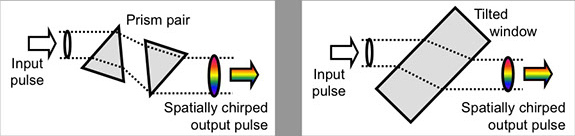
\includegraphics[width=\textwidth]{spatialchirp.png}
    \caption{Spatial chirp verursacht durch einen Prismenkompressor (links) und
        ein schiefes Glas (rechts) \cite{tutspatialchirp}}
    \label{fig:spatialchirp}
\end{figure}
\subsection{Pulse Front Tilt}
Eine weitere räumliche Verzerrung ist der sog. Pulse Front Tilt. Er gibt an, um
wie viel die Pulsfront eines Laserpulses gegenüber der optischen Achse geneigt
ist. Er wird hervorgerufen durch Winkeldispersion oder auch durch das
Durchqueren eines räumlich gechirpten Pulses durch ein lineares Medium
(\cref{fig:pft}).
\begin{figure}[]
    \centering
    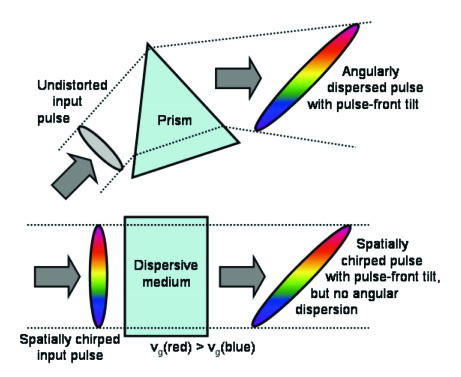
\includegraphics[width=0.5\textwidth]{pft.jpeg}
    \caption{Pulse Front Tilt verursacht durch Winkeldispersion (oben) und
        räumlichen Chirp (unten) \cite{Akturk:04}.}
    \label{fig:pft}
\end{figure}

\subsection{Prismenkrompressor}
\begin{figure}[]
    \centering
    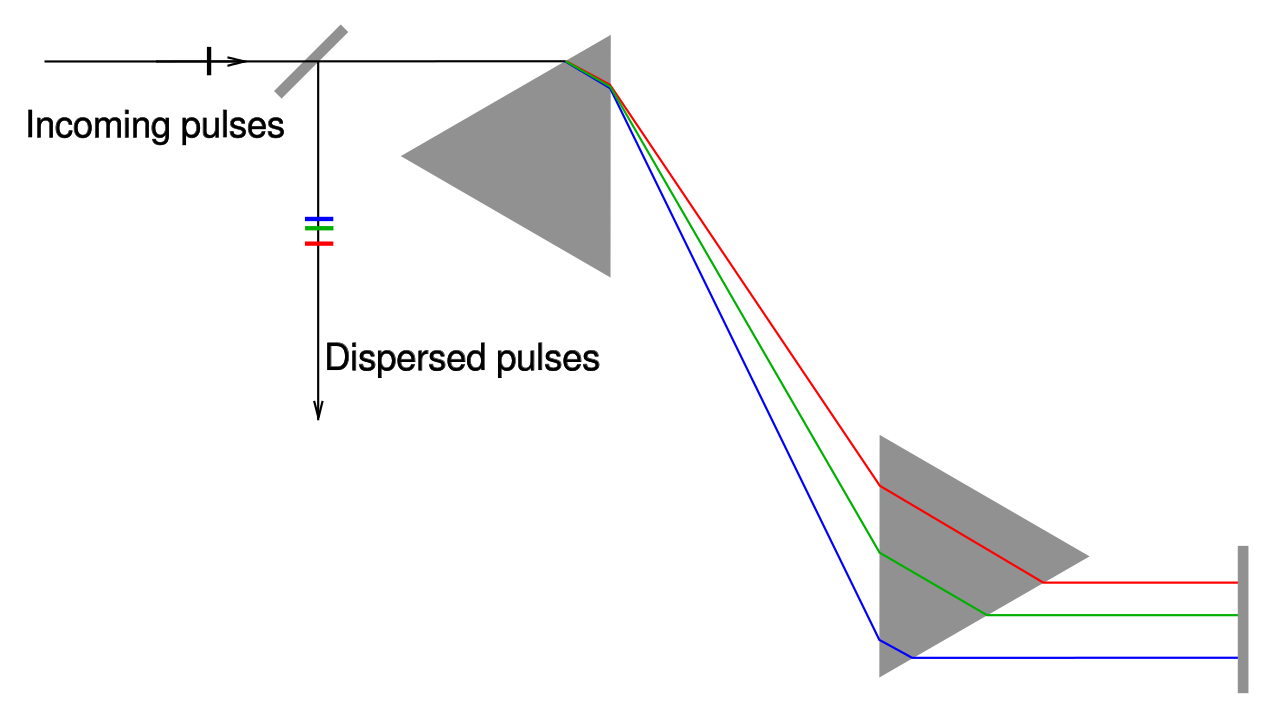
\includegraphics[width=\textwidth]{pc.png}
    \caption{Schematischer Aufbau eines Prismenkompressors. Ein ungechirpter
    Puls tritt ein und wird temporal gechirpt, da unterschiedliche Wellenlängen
    andere Propagationspfade nehmen. Bei entgegengesetztem Durchgang wird
    ersichtlich: Ein gechirpter Puls wird durch einen Prismenkompressor bei
    richtiger Einstellung ungechirpt, ``komprimiert''. Die Insertion ist definiert als der
    Abstand des Eintrittspunktes der zentralen Wellenlänge (hier grün) und der
    Spitze des zweiten Prismas .\cite{wikipc}}
    \label{fig:pc}
\end{figure}
Mithilfe des Prismenkompressors (PC) kann ein gechirpter Puls wieder zu einem
(nahezu) Fourier-limitierten Puls komprimiert werden. Der Aufbau des
Prismenkompressors ist in \cref{fig:pc} zu sehen. Der Puls durchquert zwei
Prismen, die entgegengesetzt parallel zueinander aufgestellt sind. Dabei sind
sie so positioniert, dass der Puls beim ersten Prisma gerade durch die Spitze
gelangt. Nach Snell's Gesetz verlassen die unterschiedlichen Wellenlängen
das erste Prisma in unterschiedlichen Winkeln. Dadurch durchqueren sie
unterschiedlich lange Strecken im zweiten Prisma. Durch die spezielle
Positionierung verlassen alle Wellenlängen das zweite Prisma wieder parallel,
aber mit einem räumlichen Chirp. Um diesen auszugleichen wird der Strahl an
einem Spiegel zurück reflektiert und nimmt somit den gleichen Weg erneut durch
den Prismenkompressor. Durch die unterschiedlichen Weglängen der verschiedenen
Frequenzen kann bei richtiger Positionierung des zweiten Prismas die Group
Delay Dispersion negativ werden, wodurch ein gechirpter Puls entchirpt werden
kann. Für die GDD des Prismenkompressors gilt: \cite{Diels2006}<++> 
\begin{align}
    \diff[2]{\varphi}{\omega}|_{\omega_0}=2\frac{\lambda_0^2}{2\pi c_0^2}\left[
    L_g\diff[2]{n}{\lambda}|_{\lambda_0}-(4L+\frac{L_g}{n(\lambda_0)^3})(\diff{n}{\lambda}|_{\lambda_0})^2
    \right],
    \label{eq:pc}
\end{align}
wobei $\lambda_0$ die Trägerwellenlänge, $L_g$ die Weglänge im Glas für die
Trägerwellenlänge und $L$ der Abstand der Spitzen der beiden Prismen ist. Für
symmetrisch positionierte Prismen in Brewsterwinkel-Konfiguration gilt
$L_g=2I\frac{1}{\sqrt{1+n(\lambda_0)^2}}$ mit dem Einschub (Insertion) des
zweiten Prismas $I$, welcher im Experiment mit der Millimeterschraube direkt
eingestellt wird.

\subsection{Grenouille}
Um einen zeitlichen Prozess zu messen, benötigt man einen zweiten kürzeren Prozess, um
den ersten auflösen zu können. Da ultrakurze Pulse einige Femtosekunden lang
sind, während die Elektronik auf der Nanosekundenskala agiert, ist es demnach
für solche besonders schwer, die Pulslänge zu messen. 
Es gibt verschiedene Methoden: Ein erste Ansatz ist es, mithilfe eines
Michelson-Interferrometers die Autokorrelation $A(\tau)=\int E(t)E^*(t-\tau)\d
t$ zu bestimmen. Aus der gemessenen Intensität lässt sich die grobe
Pulsstruktur rekonstruieren. Autokorrelations-Methoden haben allerdings viele
Probleme, wie die Unterschätzung der Pulslänge durch sogenannte kohärente Artefakte
\cite{swampintro}. Zusätzlich ist es unmöglich, die Phase eines ultrakurzen
Pulses mithilfe dieser Methoden zu messen.

GRENOUILLE (Grating-eliminated No-nonsense Observation Of Ultrafast Incident
Laser Light E Fields) behebt alle Probleme von Autokorrelations-Methoden und
liefert zusätzliche Informationen über den Puls: Es basiert auf dem ``Frequency
Resolved Optical Gating'' (FROG) \cite{Trebino2012}, bei dem die spektrale Intensität gegenüber
der zeitlichen Verzögerung des Auftreffens auf dem Detektor , der sogenannte
Frog trace gemessen wird. Aus diesem wird mithilfe eines Algorithmus die
Pulsdauer, die Bandbreite sowie die Phase und die spektrale Phase
rekonstruiert. Bei GRENOUILLE wird ein vereinfachter Aufbau, bestehend aus
einem Fresnelschen Biprisma und einem second-harmonic generation (SHG) Kristall
verwendet. Ein breiter SHG Kristall fächert die unterschiedlichen Wellenlängen entlang einer Dimension
auf, während das Fresnelsche Biprisma in der anderen Dimension den Puls teilt
und mit unterschiedlicher Verzögerung mit sich selbst interferieren lässt.
Dadurch entsteht der Frog trace, welcher den Puls überbestimmt. Somit lassen
sich alle relevanten Informationen eines ultrakurzen Pulses rekonstruieren
\cite{SwampOpticsFrog}. Insbesondere liefert die spektrale Phase den Chirp des Pulses. Es ist
jedoch darauf zu Achten, dass die Methode symmetrisch gegenüber der
Zeitrichtung ist und deswegen der Vorzeichen des Chirps nicht bestimmt wird.
Zusätzlich werden automatisch der Pulse Front Tilt, sowie der räumliche Chirp
gemessen. Sie spiegeln sich im Frog trace jeweils als Verschiebung auf der
Verzögerungsachse und als Scherung des Traces wider.



\section{Durchführung}
\label{sec:durchfuehrung}
\subsection{Aufbau}
Der Versuchsaufbau ist in \cref{fig:aufbau} zu sehen. Die verwendete Laserquelle
ist ein Spectra Physics Tsunami mit einer zentralen Wellenlänge von 800\;nm,
einer Durchschnittsleistung von 400\;mW, einer Pulsrate von 76\;MHz und einer
Pulsdauer von 22\;fs bei einer Bandbreite von 58\;nm. Der Strahl durchquert
zunächst eine $\lambda/2$ Platte und wird p-polarisiert. Anschließend
durchquert er den Prismenkompressor. Der Abstand der Prismen von Spitze zu
Spitze wurde gemessen und beträgt $43,2\pm0.3$\;cm. Der Prismeneinschub wird
direkt über eine Millimeterschraube variiert. Dem Laser stehen nun
drei mögliche Strahlengänge zur Verfügung, welche jeweils mit Klappspiegeln
eingestellt werden können. Pfad 1 besteht aus metallischen Spiegeln und einer
optischen Bank, auf die verschiedene Glasfenster aus BK7 oder MgF2, sowie ein
Glasspat und ein Langpass Filter geschraubt werden können. Pfad 2 besteht aus
dielektrischen Spiegeln. Auf Pfad 3 durchquert der Strahl ein Spiegelpaar mit
jeweils 5 Reflektionen. Es handelt sich hierbei um gechirpte Spiegel, was die
spätere Auswertung zeigt. Alle drei Pfade enden in dem Messinstrument, einem
Swamp Optics Grenouille (Modell 8-20-USB). Zur Justage der Strahlengänge stehen
diverse Justagespiegel, Infrarot-Irisblenden und Infrarotkarten bereit.

\begin{figure}[]
    \begin{center}
        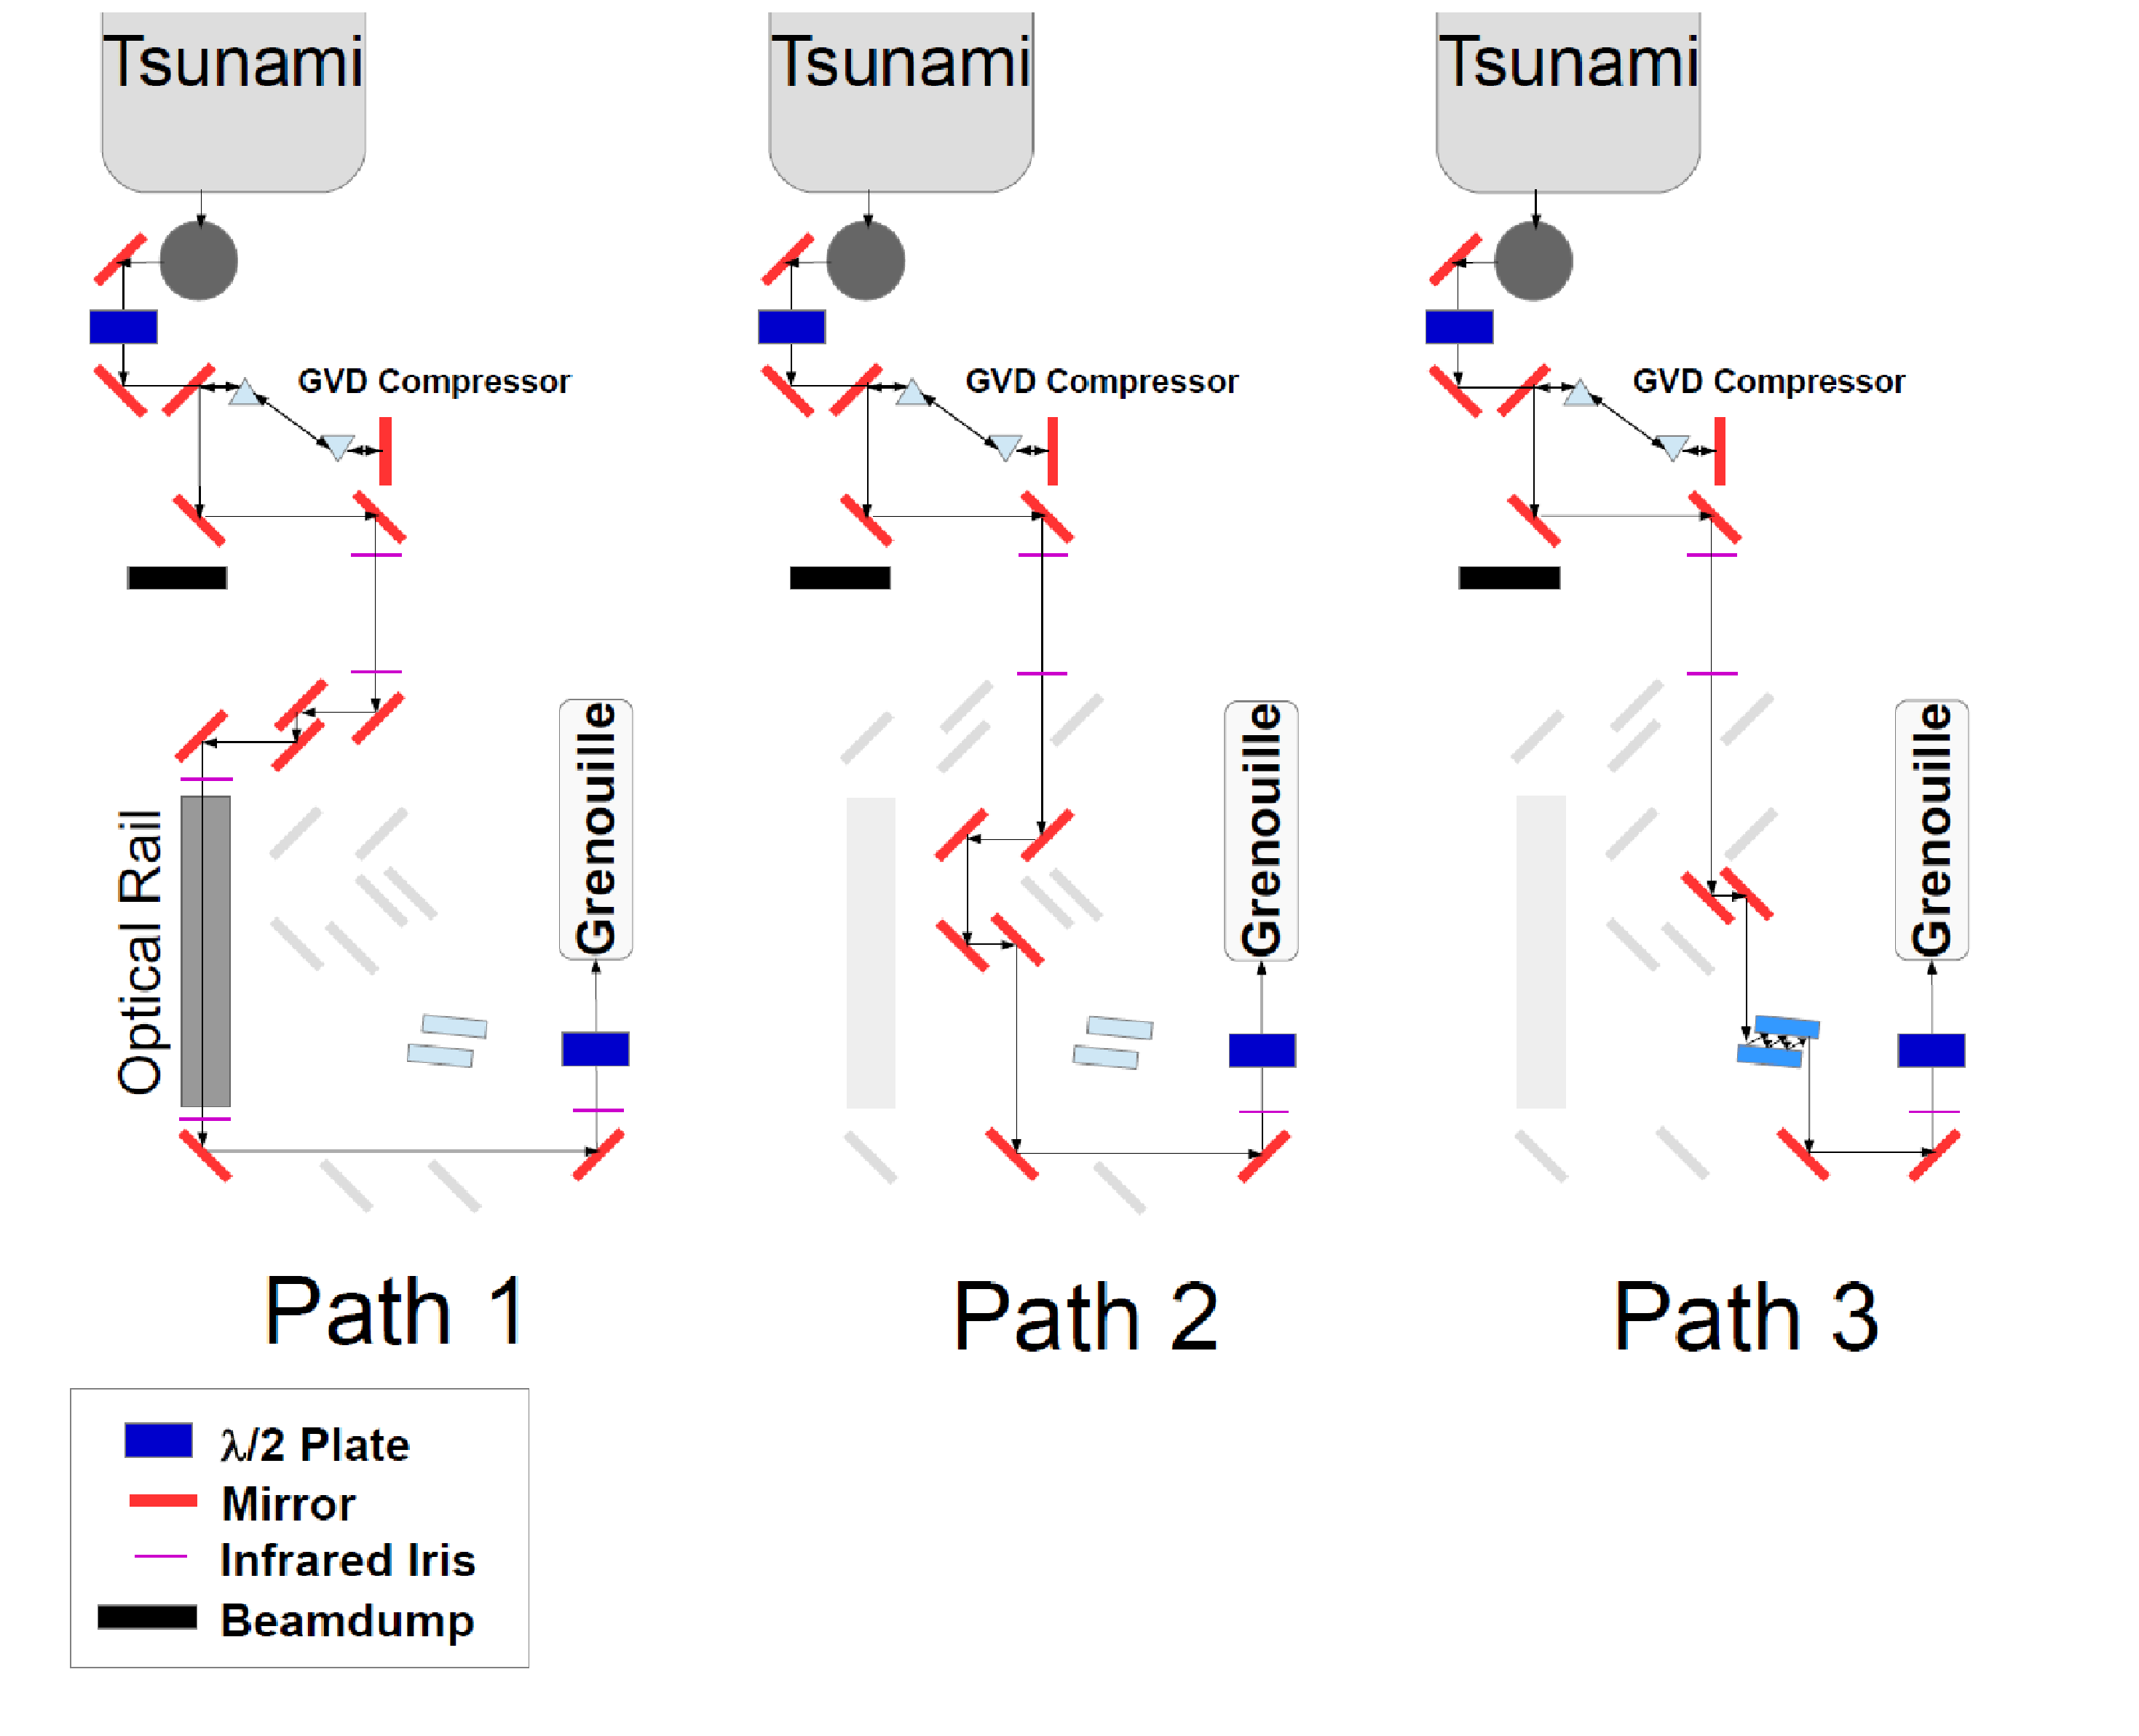
\includegraphics[width=0.7\textwidth]{aufbau1.eps}
    \end{center}
    \caption{Versuchsaufbau. Der Laser passiert zunächst eine $\lambda/2$
    Platte, anschließend den Prismenkompressor und geht dann entlang einen von
    drei möglichen Strahlengängen mit unterschiedlichen optischen Komponenten.
    Nach einer zweiten $\lambda/2$ Platte endet der Strahl im Grenouille
    Analysator \cite{fprakt}.}
    \label{fig:aufbau}
\end{figure}

\subsection{Sicherheitshinweise}
Da es sich bei dem verwendeten Laser um einen der Klasse 4 handelt, sind
zunächst einige Sicherheitshinweise zu beachten: Es müssen stets geeignete
Laserschutzbrillen getragen werden. Alle reflektierenden Objekte müssen vor dem
Versuch abgelegt werden. Es sollte auch trotz der Schutzbrillen niemals direkt
in den Laserstrahl geschaut werden. Ebenso sollte vermieden werden, mit der
Hand direkt in den Strahlengang zu fassen. Es ist besonders wichtig, dass stets
der gesamte Strahlengang des Lasers bekannt ist, bevor dieser zur Propagation
freigegeben wird. Deswegen müssen bei der Justage stets zwei Infrarotkarten und
gegebenfalls weitere Beamdumps benutzt werden, um den Strahlengang nach und nach
durch die hinzugefügten optischen Elemente zu leiten. Niemals darf ein
optisches Element ohne Blockieren des Lasers in den Strahlengang gestellt
werden, da unerwartete Reflexe auftreten können.\\
\subsection{Durchführung}
Zunächst wird der Prismenkompressor ohne zusätzliche optische Elemente
vermessen und somit auch seine optimale Position bestimmt. Dazu wird der Laser mithilfe der Irisblenden und den Justagespiegeln
auf Strahlengang 1 justiert. Bei dieser und jeder anderen Messung muss der
Laser zunächst mithilfe des space-Modus der Analysesoftware Quick-Frog der Strahl in den
Grenouille zentriert werden. Dies geschieht wieder mit Justagespiegeln und zwei
Irisblenden. Wichtig ist, dass der erste Spiegel den Strahl auf die erste
Irisblende ausrichtet, während der zweite Spiegel für die zweite Blende
verwendet wird (``beam walking''). Anschließend kann die Software auf den
time-mode gestellt werden um die Echtzeitdaten des Lasers zu sehen. Hierbei ist
auf ausreichende, aber nicht zu große Intensität des auftreffenden Strahles zu
achten, welche über die zweite $\lambda/2$ Platte unmittelbar vor dem Analysator
eingestellt werden kann.\\
Um die optimale Kompressorposition zu bestimmen, wird der Einschub über die
Millimeterschraube solange variiert, bis die gemessene Pulslänge (temporal
FWHM) minimal ist. Da der Laser bereits mit etwas Chirp aus der Quelle kommt,
wird somit garantiert, dass der komprimierte Puls die kürzeste Dauer und somit
(näherungsweise) gaußförmig und ungechirpt ist (siehe Auswertung). Dies ist der
Ausgangspunkt von allen anderen Messungen. Die Daten
werden gespeichert und die Prismenkonfiguration notiert. Anschließend werden
weitere Daten für unterschiedliche Prismenpositionen ermittelt.\\
Nun werden Daten mit
verschiedenen optischen Elementen, wie unterschiedlich dicken Gläsern aus BK7 und
MgF2, sowie einem Glasspat und einem Langpassfilter auf der optischen Bank
aufgenommen. Bei jedem optischen Element muss der Strahl erneut in den
Grenouille zentriert werden. Bei jeder Messung wird zunächst die Messung bei
optimaler Kompressorposition durchgeführt. Anschließend wird versucht, die
Pulsverbreiterungen mit dem Kompressor zu kompensieren, indem wieder die
Pulslänge minimiert wird. Die Prismenpositionen werden erneut aufgeschrieben.
Anschließend wird der Laser auf Strahlengang 2 justiert und es werden bei
optimaler Prismeneinstellung Daten für die dielektrischen Spiegel gespeichert
und erneut wird versucht die Verzerrungen zu kompensieren.
Als nächstes wird der Strahlengang 3 justiert und der Effekt der Spiegelpaare
wird bei optimaler Prismenposition aufgenommen und versucht zu kompensieren.
Nun wird die Bandbreite des Lasers verändert und die Messungen des
Prismenkompressors und der der Glasfenster werden wiederholt.
Es wurde versäumt, für die zweite Bandbreite eine neue optimale Prismenposition
zu bestimmen.


\section{Auswertung}
\label{sec:auswertung}
\subsection{Prismenkompressor}
Zunächst wird die Vermessung des Prismenkompressors analysiert. Um die Insertion $l$ des
Prismas zu bestimmen, wurde der Wert der Millimeterschraube bei der optimalen
Einstellung mit minimaler Pulsdauer (``opt'') von jenem abgezogen, bei welchem
die Bandbreite aufgrund des Abschneidens des Lasers durch Verfehlen des zweiten
Prismas geringer wurde. Dies ist jedoch eine grobe Abschätzung, da der genaue
Zeitpunkt des Verfehlens aufgrund des endlichen Laserdurchemssers willkürlich
war. Die Idee ist, dass das Abschneiden einer Insertion von $0\;$mm bedeutet.
Demnach wurden alle anderen Werte der Millimeterschraube von diesem abgezogen. 
Der optimale Einschub mit Pulsdauer ist somit $I_2=2.84$. Für die gemessene
Trägerwellenlänge bei dieser Einstellung wurde $\lambda_0=790\;$nm bestimmt. Die
Pulsdauer ergab $\tau_0=24.5\;$fs, die Bandbreite $\Delta\omega_0=46.3\;$nm,
was mit der Umrechnungsformel $\Delta\omega=\frac{2\pi\Delta\lambda}{\lambda_0^2}$ einer Kreisfrequenzbandbreite von $\Delta\omega=14.0\;$fs entspricht.
Um die Pulscharakteristiken bei optimaler Prismeneinstellung zu erkennen,
werden die für unterschiedlichen Einschub des zweiten Prismas gemessenen zeitlichen
Pulsintensitäten sowie das Spektrum verglichen. 
Die gemessene zeitliche Pulsintensität der ersten Laserausgangsbandbreite ist in
\cref{fig:temp1} in Abhängigkeit von der Insertion $I$ aufgetragen. Ebenso
eingetragen sind die gemessen Phasen $\Phi$. Es ist zu beachten, dass es sich
hier um den Absolutbetrag der Phase handelt, da das Vorzeichen aufgrund der
Zeitumkehrungsymmetrie von Grenouille keine Bedeutung hat. Um den linearen Chirp, also den Term zweiter Ordnung in \cref{eq:taylor} zu bestimmen, wird um das
Phasenmaximum bei optimale Prismeneinstellung eine Funktion mit Ansatz
$\frac{1}{2}a(x-b)^2$ gefittet. Der Term $a$ ist nach \cref{eq:taylor} die
zweite Ableitung der Phase nach der Zeit und gibt somit den zeitlichen Chirp
an. Der Term $b$ gibt an, um wie viel sich das Spektrum verschiebt. In \cref{fig:spec1} ist das vermessene Spektrum, sowie die spektralen Phasen der ersten Laserbandbreite für verschiedene $I$ aufgetragen. Wie bei den zeitlichen Intensitäten wird auch hier die Phase für die optimale Einstellung mit einem quadratischen Polynom gefittet. Der quadratische Term ist der lineare Chirp,
welcher für eine Pulsverbreiterung im Zeitraum verantwortlich ist.
Dieser muss allerdings noch in fs$^2$ umgerechnet werden. Nach \cref{eq:gvd}
und der Kettenregel gilt $\diff[2]{\varphi}{\omega}=\frac{\lambda^2}{2\pi c)^2}\left(
\lambda^2\diff[2]{\varphi}{\lambda}+2\lambda\diff{\varphi}{\lambda} \right)$.
Der zweite Term kann vernachlässigt werden, da um ein Extremum gefittet wird. Man
erhält eine Gruppengeschwindigkeitsdispersion von GDD$_0=20.26\pm6\;$fs$^2$.
Gleiches wird ebenfalls für die zweite Ausgangs-Bandbreite von
$\braket{\lambda^2}=27\pm1\;$nm berechnet. Die Intensität und das Spektrum mit Phasen
ist jeweils in \cref{fig:temp2} und \cref{fig:spec2} aufgetragen. Es wurde
versäumt, für diese zweite Bandbreite eine neue optimale
Prismenkompressor-Position zu bestimmten, demnach ist mit ``opt'' hier weiterhin
die optimale Position der ersten Bandbreite bezeichnet.
Die Ergebnisse der Regressionen sind in Tabelle \cref{tab:fits}
zusammengefasst. Die gemessene GDD ist besonders für die erste Bandbreite sehr
gering im Vergleich zu den GDDs des Prismenkompressors (s.u.). Demnach ist der
Puls nach dem Prismenkompressor in optimaler Einstellung nahezu gaußförmig.


\begin{table}
    \centering
    \begin{tabular}[]{||c|c|c||c|c|c||}
        \hline
        &\multicolumn{2}{|c||}{Intensität}&\multicolumn{3}{|c||}{Spektrum}\\\hline\hline
        &$a\,\{\diff[2]{\Phi}{t}\}$\;[fs$^{-2}$]&$b\, \{t_0\}\;$[fs]&$a\,\{\diff[2]{\varphi}{\lambda}\}$\;[nm$^{-2}$]&$\diff[2]{\varphi}{\omega}$\;[fs$^{-2}$]&$b\, \{\lambda_0\}\;$[nm]\\\hline
       $\Delta\lambda_1$&$0.001507\pm0.000014$&$-0.001793\pm0.000054$&$0.000727\pm0.000021$&$20\pm6$&$793.88\pm0.60$\\\hline
       $\Delta\lambda_2$&$0.000555\pm0.000003$&$1.612\pm0.034$&$0.001815\pm0.000046$&$51\pm13$&$797.81\pm0.11$\\\hline
    \end{tabular}
    \caption{Ergebnisse der quadratischen Fits für die Phase und die
    spektrale Phase der optimalen Prismenkonfiguration.
    $\Delta\lambda_1=55\pm1$\;nm, $\Delta\lambda_2=27\pm1$\;nm.}
    \label{tab:fits}
\end{table}
Als nächstes wird die GDD des Prismenkompressors analysiert. Hierfür wird
zunächst die theoretische GDD nach \cref{eq:pc} zusammen mit
\cref{eq:sellmeier} berechnet. Das PC-Material ist N-LAK21. Die
Ungenauigkeiten werden mit den Ungenauigkeiten $\sigma_L=3\;$mm,
$\sigma_{l_2}=0.1\;$mm und $\sigma_{\Delta_{\lambda}}=1\;$mm nach der gauß'schem
Fehlerfortpflanzungsformel berechnet. Da nach der vorherigen Auswertung bei
optimaler PC Einstellung ein nahezu ungechirpter Puls vorliegt, wird der
zugehörige theoretische GDD Wert des PC's von den anderen abgezogen. Als
Resultat erhält man die GDD, die für die Pulsverbreiterung verantwortlich ist.
Somit lässt sich die theoretische GDD des PC's ausrechnen. Ebenso wird aus den
Messungen mit Kompensation die tatsächlich eingestellte GDD für die
Kompensation berechnet.
Aus der GDD wird schließlich die neue Pulslänge nach
\ref{eq:pulsverbreiterung} bestimmt, wobei eine Ungenauigkeit der Pulslänge von
$\sigma_\tau=3$\;fs angenommen wird. Die theoretischen und die tatsächlich
gemessenen Pulslängen in Abhängigkeit der GDD des Prismenkompressors für beide
Bandbreiten sind in \cref{fig:pckieran1,fig:pckieran2} zu sehen. Hierbei wurden
beide Größen quadriert, um nach \cref{eq:pulsverbreiterung} einen linearen
Zusammenhang zu bekommen. Für die erste
Bandbreite sind die Messwerte in guter Übereinstimmung mit der Theorie.
Lediglich die letzten beiden Messpunkte, bei denen der Laser bereits partiell
vom Prisma abgeschnitten wurde, zeigen eine größere Abweichung. Für die zweite
Bandbreite sind die Ergebnisse nur qualitativ korrekt, was aufgrund der
Versäumung des Messens einer neuen optimalen Prismenposition zu erwarten ist.

\begin{figure}[]
    \centering
    % GNUPLOT: LaTeX picture with Postscript
\begingroup
  \makeatletter
  \providecommand\color[2][]{%
    \GenericError{(gnuplot) \space\space\space\@spaces}{%
      Package color not loaded in conjunction with
      terminal option `colourtext'%
    }{See the gnuplot documentation for explanation.%
    }{Either use 'blacktext' in gnuplot or load the package
      color.sty in LaTeX.}%
    \renewcommand\color[2][]{}%
  }%
  \providecommand\includegraphics[2][]{%
    \GenericError{(gnuplot) \space\space\space\@spaces}{%
      Package graphicx or graphics not loaded%
    }{See the gnuplot documentation for explanation.%
    }{The gnuplot epslatex terminal needs graphicx.sty or graphics.sty.}%
    \renewcommand\includegraphics[2][]{}%
  }%
  \providecommand\rotatebox[2]{#2}%
  \@ifundefined{ifGPcolor}{%
    \newif\ifGPcolor
    \GPcolortrue
  }{}%
  \@ifundefined{ifGPblacktext}{%
    \newif\ifGPblacktext
    \GPblacktexttrue
  }{}%
  % define a \g@addto@macro without @ in the name:
  \let\gplgaddtomacro\g@addto@macro
  % define empty templates for all commands taking text:
  \gdef\gplbacktext{}%
  \gdef\gplfronttext{}%
  \makeatother
  \ifGPblacktext
    % no textcolor at all
    \def\colorrgb#1{}%
    \def\colorgray#1{}%
  \else
    % gray or color?
    \ifGPcolor
      \def\colorrgb#1{\color[rgb]{#1}}%
      \def\colorgray#1{\color[gray]{#1}}%
      \expandafter\def\csname LTw\endcsname{\color{white}}%
      \expandafter\def\csname LTb\endcsname{\color{black}}%
      \expandafter\def\csname LTa\endcsname{\color{black}}%
      \expandafter\def\csname LT0\endcsname{\color[rgb]{1,0,0}}%
      \expandafter\def\csname LT1\endcsname{\color[rgb]{0,1,0}}%
      \expandafter\def\csname LT2\endcsname{\color[rgb]{0,0,1}}%
      \expandafter\def\csname LT3\endcsname{\color[rgb]{1,0,1}}%
      \expandafter\def\csname LT4\endcsname{\color[rgb]{0,1,1}}%
      \expandafter\def\csname LT5\endcsname{\color[rgb]{1,1,0}}%
      \expandafter\def\csname LT6\endcsname{\color[rgb]{0,0,0}}%
      \expandafter\def\csname LT7\endcsname{\color[rgb]{1,0.3,0}}%
      \expandafter\def\csname LT8\endcsname{\color[rgb]{0.5,0.5,0.5}}%
    \else
      % gray
      \def\colorrgb#1{\color{black}}%
      \def\colorgray#1{\color[gray]{#1}}%
      \expandafter\def\csname LTw\endcsname{\color{white}}%
      \expandafter\def\csname LTb\endcsname{\color{black}}%
      \expandafter\def\csname LTa\endcsname{\color{black}}%
      \expandafter\def\csname LT0\endcsname{\color{black}}%
      \expandafter\def\csname LT1\endcsname{\color{black}}%
      \expandafter\def\csname LT2\endcsname{\color{black}}%
      \expandafter\def\csname LT3\endcsname{\color{black}}%
      \expandafter\def\csname LT4\endcsname{\color{black}}%
      \expandafter\def\csname LT5\endcsname{\color{black}}%
      \expandafter\def\csname LT6\endcsname{\color{black}}%
      \expandafter\def\csname LT7\endcsname{\color{black}}%
      \expandafter\def\csname LT8\endcsname{\color{black}}%
    \fi
  \fi
    \setlength{\unitlength}{0.0500bp}%
    \ifx\gptboxheight\undefined%
      \newlength{\gptboxheight}%
      \newlength{\gptboxwidth}%
      \newsavebox{\gptboxtext}%
    \fi%
    \setlength{\fboxrule}{0.5pt}%
    \setlength{\fboxsep}{1pt}%
\begin{picture}(7200.00,5040.00)%
    \gplgaddtomacro\gplbacktext{%
      \csname LTb\endcsname%
      \put(814,704){\makebox(0,0)[r]{\strut{}$0$}}%
      \put(814,1518){\makebox(0,0)[r]{\strut{}$0.2$}}%
      \put(814,2332){\makebox(0,0)[r]{\strut{}$0.4$}}%
      \put(814,3147){\makebox(0,0)[r]{\strut{}$0.6$}}%
      \put(814,3961){\makebox(0,0)[r]{\strut{}$0.8$}}%
      \put(814,4775){\makebox(0,0)[r]{\strut{}$1$}}%
      \put(946,484){\makebox(0,0){\strut{}$-80$}}%
      \put(1585,484){\makebox(0,0){\strut{}$-60$}}%
      \put(2223,484){\makebox(0,0){\strut{}$-40$}}%
      \put(2862,484){\makebox(0,0){\strut{}$-20$}}%
      \put(3501,484){\makebox(0,0){\strut{}$0$}}%
      \put(4139,484){\makebox(0,0){\strut{}$20$}}%
      \put(4778,484){\makebox(0,0){\strut{}$40$}}%
      \put(5416,484){\makebox(0,0){\strut{}$60$}}%
      \put(6055,484){\makebox(0,0){\strut{}$80$}}%
      \put(6187,1111){\makebox(0,0)[l]{\strut{}$-4$}}%
      \put(6187,1925){\makebox(0,0)[l]{\strut{}$-2$}}%
      \put(6187,2740){\makebox(0,0)[l]{\strut{}$0$}}%
      \put(6187,3554){\makebox(0,0)[l]{\strut{}$2$}}%
      \put(6187,4368){\makebox(0,0)[l]{\strut{}$4$}}%
    }%
    \gplgaddtomacro\gplfronttext{%
      \csname LTb\endcsname%
      \put(176,2739){\rotatebox{-270}{\makebox(0,0){\strut{}Intensität $I$}}}%
      \put(6692,2739){\rotatebox{-270}{\makebox(0,0){\strut{}Phase $\Phi$ [rad]}}}%
      \put(3500,154){\makebox(0,0){\strut{}Zeit $t$ [fs]}}%
      \csname LTb\endcsname%
      \put(5068,4602){\makebox(0,0)[r]{\strut{}\tiny$I:2.04\;\text{nm}$}}%
      \csname LTb\endcsname%
      \put(5068,4382){\makebox(0,0)[r]{\strut{}\tiny$I:2.5\;\text{nm}$}}%
      \csname LTb\endcsname%
      \put(5068,4162){\makebox(0,0)[r]{\strut{}\tiny$I:1.75\;\text{nm}$}}%
      \csname LTb\endcsname%
      \put(5068,3942){\makebox(0,0)[r]{\strut{}\tiny$I:1.3\;\text{nm}$}}%
      \csname LTb\endcsname%
      \put(5068,3722){\makebox(0,0)[r]{\strut{}\tiny$I:0.7\;\text{nm}$}}%
      \csname LTb\endcsname%
      \put(5068,3502){\makebox(0,0)[r]{\strut{}\tiny$I:0\;\text{nm}$}}%
      \csname LTb\endcsname%
      \put(5068,3282){\makebox(0,0)[r]{\strut{}\tiny$I:2.84\;\text{nm (opt)}$}}%
      \csname LTb\endcsname%
      \put(5068,3062){\makebox(0,0)[r]{\strut{}\tiny$\Phi:2.04\;\text{nm}$}}%
      \csname LTb\endcsname%
      \put(5068,2842){\makebox(0,0)[r]{\strut{}\tiny$\Phi:2.5\;\text{nm}$}}%
      \csname LTb\endcsname%
      \put(5068,2622){\makebox(0,0)[r]{\strut{}\tiny$\Phi:1.75\;\text{nm}$}}%
      \csname LTb\endcsname%
      \put(5068,2402){\makebox(0,0)[r]{\strut{}\tiny$\Phi:1.3\;\text{nm}$}}%
      \csname LTb\endcsname%
      \put(5068,2182){\makebox(0,0)[r]{\strut{}\tiny$\Phi:0.7\;\text{nm}$}}%
      \csname LTb\endcsname%
      \put(5068,1962){\makebox(0,0)[r]{\strut{}\tiny$\Phi:0\;\text{nm}$}}%
      \csname LTb\endcsname%
      \put(5068,1742){\makebox(0,0)[r]{\strut{}\tiny$\Phi:2.84\;\text{nm (opt)}$}}%
      \csname LTb\endcsname%
      \put(5068,1522){\makebox(0,0)[r]{\strut{}\small$\text{fit}$}}%
    }%
    \gplbacktext
    \put(0,0){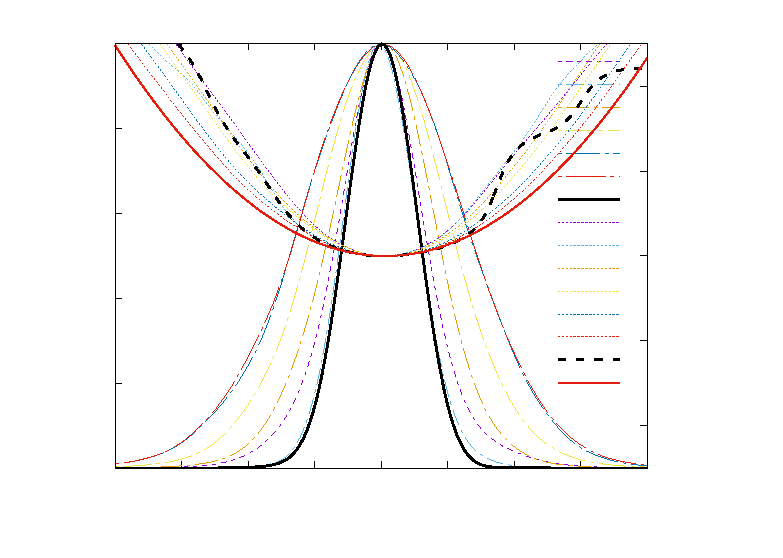
\includegraphics{temp1}}%
    \gplfronttext
  \end{picture}%
\endgroup

    \caption{Intensität für verschiedene Einschübe $l$ mit Phase. Um die
    optimale Phase wurde ein Polynomfit zweiter Ordnung
    gefittet. $\Delta\lambda=55\pm1$.}
    \label{fig:temp1}
\end{figure}
\begin{figure}[]
    \centering
    % GNUPLOT: LaTeX picture with Postscript
\begingroup
  \makeatletter
  \providecommand\color[2][]{%
    \GenericError{(gnuplot) \space\space\space\@spaces}{%
      Package color not loaded in conjunction with
      terminal option `colourtext'%
    }{See the gnuplot documentation for explanation.%
    }{Either use 'blacktext' in gnuplot or load the package
      color.sty in LaTeX.}%
    \renewcommand\color[2][]{}%
  }%
  \providecommand\includegraphics[2][]{%
    \GenericError{(gnuplot) \space\space\space\@spaces}{%
      Package graphicx or graphics not loaded%
    }{See the gnuplot documentation for explanation.%
    }{The gnuplot epslatex terminal needs graphicx.sty or graphics.sty.}%
    \renewcommand\includegraphics[2][]{}%
  }%
  \providecommand\rotatebox[2]{#2}%
  \@ifundefined{ifGPcolor}{%
    \newif\ifGPcolor
    \GPcolortrue
  }{}%
  \@ifundefined{ifGPblacktext}{%
    \newif\ifGPblacktext
    \GPblacktexttrue
  }{}%
  % define a \g@addto@macro without @ in the name:
  \let\gplgaddtomacro\g@addto@macro
  % define empty templates for all commands taking text:
  \gdef\gplbacktext{}%
  \gdef\gplfronttext{}%
  \makeatother
  \ifGPblacktext
    % no textcolor at all
    \def\colorrgb#1{}%
    \def\colorgray#1{}%
  \else
    % gray or color?
    \ifGPcolor
      \def\colorrgb#1{\color[rgb]{#1}}%
      \def\colorgray#1{\color[gray]{#1}}%
      \expandafter\def\csname LTw\endcsname{\color{white}}%
      \expandafter\def\csname LTb\endcsname{\color{black}}%
      \expandafter\def\csname LTa\endcsname{\color{black}}%
      \expandafter\def\csname LT0\endcsname{\color[rgb]{1,0,0}}%
      \expandafter\def\csname LT1\endcsname{\color[rgb]{0,1,0}}%
      \expandafter\def\csname LT2\endcsname{\color[rgb]{0,0,1}}%
      \expandafter\def\csname LT3\endcsname{\color[rgb]{1,0,1}}%
      \expandafter\def\csname LT4\endcsname{\color[rgb]{0,1,1}}%
      \expandafter\def\csname LT5\endcsname{\color[rgb]{1,1,0}}%
      \expandafter\def\csname LT6\endcsname{\color[rgb]{0,0,0}}%
      \expandafter\def\csname LT7\endcsname{\color[rgb]{1,0.3,0}}%
      \expandafter\def\csname LT8\endcsname{\color[rgb]{0.5,0.5,0.5}}%
    \else
      % gray
      \def\colorrgb#1{\color{black}}%
      \def\colorgray#1{\color[gray]{#1}}%
      \expandafter\def\csname LTw\endcsname{\color{white}}%
      \expandafter\def\csname LTb\endcsname{\color{black}}%
      \expandafter\def\csname LTa\endcsname{\color{black}}%
      \expandafter\def\csname LT0\endcsname{\color{black}}%
      \expandafter\def\csname LT1\endcsname{\color{black}}%
      \expandafter\def\csname LT2\endcsname{\color{black}}%
      \expandafter\def\csname LT3\endcsname{\color{black}}%
      \expandafter\def\csname LT4\endcsname{\color{black}}%
      \expandafter\def\csname LT5\endcsname{\color{black}}%
      \expandafter\def\csname LT6\endcsname{\color{black}}%
      \expandafter\def\csname LT7\endcsname{\color{black}}%
      \expandafter\def\csname LT8\endcsname{\color{black}}%
    \fi
  \fi
    \setlength{\unitlength}{0.0500bp}%
    \ifx\gptboxheight\undefined%
      \newlength{\gptboxheight}%
      \newlength{\gptboxwidth}%
      \newsavebox{\gptboxtext}%
    \fi%
    \setlength{\fboxrule}{0.5pt}%
    \setlength{\fboxsep}{1pt}%
\begin{picture}(7200.00,5040.00)%
    \gplgaddtomacro\gplbacktext{%
      \csname LTb\endcsname%
      \put(814,704){\makebox(0,0)[r]{\strut{}$0$}}%
      \put(814,1518){\makebox(0,0)[r]{\strut{}$0.2$}}%
      \put(814,2332){\makebox(0,0)[r]{\strut{}$0.4$}}%
      \put(814,3147){\makebox(0,0)[r]{\strut{}$0.6$}}%
      \put(814,3961){\makebox(0,0)[r]{\strut{}$0.8$}}%
      \put(814,4775){\makebox(0,0)[r]{\strut{}$1$}}%
      \put(946,484){\makebox(0,0){\strut{}$740$}}%
      \put(1875,484){\makebox(0,0){\strut{}$760$}}%
      \put(2804,484){\makebox(0,0){\strut{}$780$}}%
      \put(3733,484){\makebox(0,0){\strut{}$800$}}%
      \put(4662,484){\makebox(0,0){\strut{}$820$}}%
      \put(5591,484){\makebox(0,0){\strut{}$840$}}%
      \put(6187,704){\makebox(0,0)[l]{\strut{}$-3$}}%
      \put(6187,1383){\makebox(0,0)[l]{\strut{}$-2$}}%
      \put(6187,2061){\makebox(0,0)[l]{\strut{}$-1$}}%
      \put(6187,2740){\makebox(0,0)[l]{\strut{}$0$}}%
      \put(6187,3418){\makebox(0,0)[l]{\strut{}$1$}}%
      \put(6187,4097){\makebox(0,0)[l]{\strut{}$2$}}%
      \put(6187,4775){\makebox(0,0)[l]{\strut{}$3$}}%
    }%
    \gplgaddtomacro\gplfronttext{%
      \csname LTb\endcsname%
      \put(176,2739){\rotatebox{-270}{\makebox(0,0){\strut{}Spektrale Intensität $S$}}}%
      \put(6692,2739){\rotatebox{-270}{\makebox(0,0){\strut{}Phase [rad]}}}%
      \put(3500,154){\makebox(0,0){\strut{}Wellenllänge $\lambda$ [nm]}}%
      \csname LTb\endcsname%
      \put(5068,4602){\makebox(0,0)[r]{\strut{}\tiny$S-$2.04\;\text{nm}}}%
      \csname LTb\endcsname%
      \put(5068,4382){\makebox(0,0)[r]{\strut{}\tiny$S-$2.5\;\text{nm}}}%
      \csname LTb\endcsname%
      \put(5068,4162){\makebox(0,0)[r]{\strut{}\tiny$S-$1.75\;\text{nm}}}%
      \csname LTb\endcsname%
      \put(5068,3942){\makebox(0,0)[r]{\strut{}\tiny$S-$1.3\;\text{nm}}}%
      \csname LTb\endcsname%
      \put(5068,3722){\makebox(0,0)[r]{\strut{}\tiny$S-$0.7\;\text{nm}}}%
      \csname LTb\endcsname%
      \put(5068,3502){\makebox(0,0)[r]{\strut{}\tiny$S-$0\;\text{nm}}}%
      \csname LTb\endcsname%
      \put(5068,3282){\makebox(0,0)[r]{\strut{}\tiny$S-$2.84$\;\text{nm (opt)}$}}%
      \csname LTb\endcsname%
      \put(5068,3062){\makebox(0,0)[r]{\strut{}\tiny$\Phi-$2.04$\;\text{nm}$}}%
      \csname LTb\endcsname%
      \put(5068,2842){\makebox(0,0)[r]{\strut{}\tiny$\Phi-$2.5$\;\text{nm}$}}%
      \csname LTb\endcsname%
      \put(5068,2622){\makebox(0,0)[r]{\strut{}\tiny$\Phi-$1.75$\;\text{nm}$}}%
      \csname LTb\endcsname%
      \put(5068,2402){\makebox(0,0)[r]{\strut{}\tiny$\Phi-$1.3$\;\text{nm}$}}%
      \csname LTb\endcsname%
      \put(5068,2182){\makebox(0,0)[r]{\strut{}\tiny$\Phi-$0.7$\;\text{nm}$}}%
      \csname LTb\endcsname%
      \put(5068,1962){\makebox(0,0)[r]{\strut{}\tiny$\Phi-$0$\;\text{nm}$}}%
      \csname LTb\endcsname%
      \put(5068,1742){\makebox(0,0)[r]{\strut{}\tiny$\Phi-2.84$\;\text{nm (opt)}$}}%
      \csname LTb\endcsname%
      \put(5068,1522){\makebox(0,0)[r]{\strut{}fit}}%
    }%
    \gplbacktext
    \put(0,0){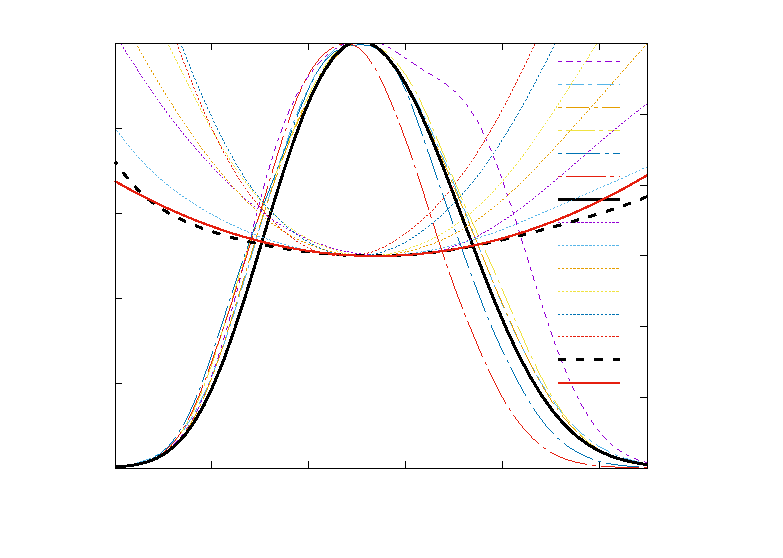
\includegraphics{spec1}}%
    \gplfronttext
  \end{picture}%
\endgroup

    \caption{Spektrale Intensität für verschiedene Einschübe $l$ mit spektraler Phase. Um die
    optimale Phase wurde ein Polynomfit zweiter Ordnung gefittet. $\Delta\lambda=55\pm1$.}
    \label{fig:spec1}
\end{figure}
\begin{figure}[]
    \centering
    % GNUPLOT: LaTeX picture with Postscript
\begingroup
  \makeatletter
  \providecommand\color[2][]{%
    \GenericError{(gnuplot) \space\space\space\@spaces}{%
      Package color not loaded in conjunction with
      terminal option `colourtext'%
    }{See the gnuplot documentation for explanation.%
    }{Either use 'blacktext' in gnuplot or load the package
      color.sty in LaTeX.}%
    \renewcommand\color[2][]{}%
  }%
  \providecommand\includegraphics[2][]{%
    \GenericError{(gnuplot) \space\space\space\@spaces}{%
      Package graphicx or graphics not loaded%
    }{See the gnuplot documentation for explanation.%
    }{The gnuplot epslatex terminal needs graphicx.sty or graphics.sty.}%
    \renewcommand\includegraphics[2][]{}%
  }%
  \providecommand\rotatebox[2]{#2}%
  \@ifundefined{ifGPcolor}{%
    \newif\ifGPcolor
    \GPcolortrue
  }{}%
  \@ifundefined{ifGPblacktext}{%
    \newif\ifGPblacktext
    \GPblacktexttrue
  }{}%
  % define a \g@addto@macro without @ in the name:
  \let\gplgaddtomacro\g@addto@macro
  % define empty templates for all commands taking text:
  \gdef\gplbacktext{}%
  \gdef\gplfronttext{}%
  \makeatother
  \ifGPblacktext
    % no textcolor at all
    \def\colorrgb#1{}%
    \def\colorgray#1{}%
  \else
    % gray or color?
    \ifGPcolor
      \def\colorrgb#1{\color[rgb]{#1}}%
      \def\colorgray#1{\color[gray]{#1}}%
      \expandafter\def\csname LTw\endcsname{\color{white}}%
      \expandafter\def\csname LTb\endcsname{\color{black}}%
      \expandafter\def\csname LTa\endcsname{\color{black}}%
      \expandafter\def\csname LT0\endcsname{\color[rgb]{1,0,0}}%
      \expandafter\def\csname LT1\endcsname{\color[rgb]{0,1,0}}%
      \expandafter\def\csname LT2\endcsname{\color[rgb]{0,0,1}}%
      \expandafter\def\csname LT3\endcsname{\color[rgb]{1,0,1}}%
      \expandafter\def\csname LT4\endcsname{\color[rgb]{0,1,1}}%
      \expandafter\def\csname LT5\endcsname{\color[rgb]{1,1,0}}%
      \expandafter\def\csname LT6\endcsname{\color[rgb]{0,0,0}}%
      \expandafter\def\csname LT7\endcsname{\color[rgb]{1,0.3,0}}%
      \expandafter\def\csname LT8\endcsname{\color[rgb]{0.5,0.5,0.5}}%
    \else
      % gray
      \def\colorrgb#1{\color{black}}%
      \def\colorgray#1{\color[gray]{#1}}%
      \expandafter\def\csname LTw\endcsname{\color{white}}%
      \expandafter\def\csname LTb\endcsname{\color{black}}%
      \expandafter\def\csname LTa\endcsname{\color{black}}%
      \expandafter\def\csname LT0\endcsname{\color{black}}%
      \expandafter\def\csname LT1\endcsname{\color{black}}%
      \expandafter\def\csname LT2\endcsname{\color{black}}%
      \expandafter\def\csname LT3\endcsname{\color{black}}%
      \expandafter\def\csname LT4\endcsname{\color{black}}%
      \expandafter\def\csname LT5\endcsname{\color{black}}%
      \expandafter\def\csname LT6\endcsname{\color{black}}%
      \expandafter\def\csname LT7\endcsname{\color{black}}%
      \expandafter\def\csname LT8\endcsname{\color{black}}%
    \fi
  \fi
    \setlength{\unitlength}{0.0500bp}%
    \ifx\gptboxheight\undefined%
      \newlength{\gptboxheight}%
      \newlength{\gptboxwidth}%
      \newsavebox{\gptboxtext}%
    \fi%
    \setlength{\fboxrule}{0.5pt}%
    \setlength{\fboxsep}{1pt}%
\begin{picture}(7200.00,5040.00)%
    \gplgaddtomacro\gplbacktext{%
      \csname LTb\endcsname%
      \put(814,704){\makebox(0,0)[r]{\strut{}$0$}}%
      \put(814,1518){\makebox(0,0)[r]{\strut{}$0.2$}}%
      \put(814,2332){\makebox(0,0)[r]{\strut{}$0.4$}}%
      \put(814,3147){\makebox(0,0)[r]{\strut{}$0.6$}}%
      \put(814,3961){\makebox(0,0)[r]{\strut{}$0.8$}}%
      \put(814,4775){\makebox(0,0)[r]{\strut{}$1$}}%
      \put(946,484){\makebox(0,0){\strut{}$-80$}}%
      \put(1585,484){\makebox(0,0){\strut{}$-60$}}%
      \put(2223,484){\makebox(0,0){\strut{}$-40$}}%
      \put(2862,484){\makebox(0,0){\strut{}$-20$}}%
      \put(3501,484){\makebox(0,0){\strut{}$0$}}%
      \put(4139,484){\makebox(0,0){\strut{}$20$}}%
      \put(4778,484){\makebox(0,0){\strut{}$40$}}%
      \put(5416,484){\makebox(0,0){\strut{}$60$}}%
      \put(6055,484){\makebox(0,0){\strut{}$80$}}%
      \put(6187,1111){\makebox(0,0)[l]{\strut{}$-4$}}%
      \put(6187,1925){\makebox(0,0)[l]{\strut{}$-2$}}%
      \put(6187,2740){\makebox(0,0)[l]{\strut{}$0$}}%
      \put(6187,3554){\makebox(0,0)[l]{\strut{}$2$}}%
      \put(6187,4368){\makebox(0,0)[l]{\strut{}$4$}}%
    }%
    \gplgaddtomacro\gplfronttext{%
      \csname LTb\endcsname%
      \put(176,2739){\rotatebox{-270}{\makebox(0,0){\strut{}Intensität $I$}}}%
      \put(6692,2739){\rotatebox{-270}{\makebox(0,0){\strut{}Phase $\Phi$ [rad]}}}%
      \put(3500,154){\makebox(0,0){\strut{}Zeit $t$ [fs]}}%
      \csname LTb\endcsname%
      \put(5068,4602){\makebox(0,0)[r]{\strut{}\tiny$I:0.95\;\text{nm}$}}%
      \csname LTb\endcsname%
      \put(5068,4382){\makebox(0,0)[r]{\strut{}\tiny$I:1.45\;\text{nm}$}}%
      \csname LTb\endcsname%
      \put(5068,4162){\makebox(0,0)[r]{\strut{}\tiny$I:1.95\;\text{nm}$}}%
      \csname LTb\endcsname%
      \put(5068,3942){\makebox(0,0)[r]{\strut{}\tiny$I:2.45\;\text{nm}$}}%
      \csname LTb\endcsname%
      \put(5068,3722){\makebox(0,0)[r]{\strut{}\tiny$I:2.84\;\text{nm}$}}%
      \csname LTb\endcsname%
      \put(5068,3502){\makebox(0,0)[r]{\strut{}\tiny$I:2.84\;\text{nm (opt)}$}}%
      \csname LTb\endcsname%
      \put(5068,3282){\makebox(0,0)[r]{\strut{}\tiny$\Phi:0.95\;\text{nm}$}}%
      \csname LTb\endcsname%
      \put(5068,3062){\makebox(0,0)[r]{\strut{}\tiny$\Phi:1.45\;\text{nm}$}}%
      \csname LTb\endcsname%
      \put(5068,2842){\makebox(0,0)[r]{\strut{}\tiny$\Phi:1.95\;\text{nm}$}}%
      \csname LTb\endcsname%
      \put(5068,2622){\makebox(0,0)[r]{\strut{}\tiny$\Phi:2.45\;\text{nm}$}}%
      \csname LTb\endcsname%
      \put(5068,2402){\makebox(0,0)[r]{\strut{}\tiny$\Phi:2.84\;\text{nm}$}}%
      \csname LTb\endcsname%
      \put(5068,2182){\makebox(0,0)[r]{\strut{}\tiny$\Phi:2.84\;\text{nm (opt)}$}}%
      \csname LTb\endcsname%
      \put(5068,1962){\makebox(0,0)[r]{\strut{}\small$\text{fit}$}}%
    }%
    \gplbacktext
    \put(0,0){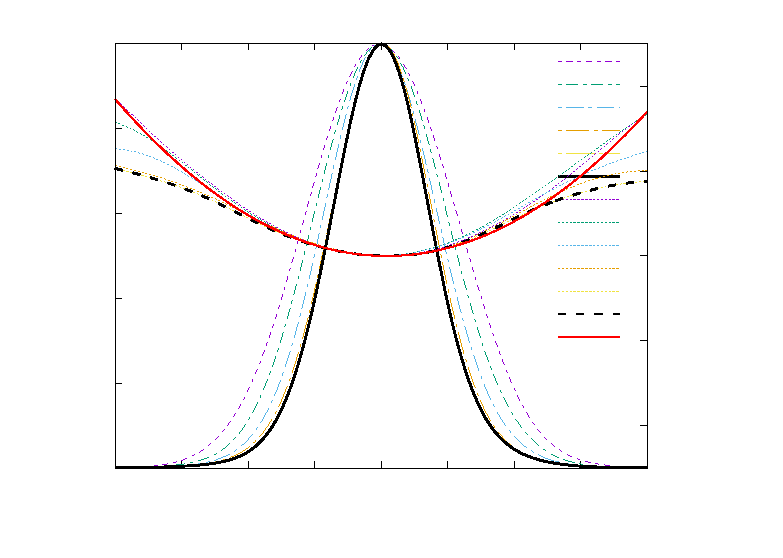
\includegraphics{temp2}}%
    \gplfronttext
  \end{picture}%
\endgroup

    \caption{Intensität für verschiedene Einschübe $l$ mit Phase. Um die
    optimale Phase wurde ein Polynomfit zweiter Ordnung gefittet. $\Delta\lambda=27\pm1$.}
    \label{fig:temp2}
\end{figure}
\begin{figure}[]
    \centering
    % GNUPLOT: LaTeX picture with Postscript
\begingroup
  \makeatletter
  \providecommand\color[2][]{%
    \GenericError{(gnuplot) \space\space\space\@spaces}{%
      Package color not loaded in conjunction with
      terminal option `colourtext'%
    }{See the gnuplot documentation for explanation.%
    }{Either use 'blacktext' in gnuplot or load the package
      color.sty in LaTeX.}%
    \renewcommand\color[2][]{}%
  }%
  \providecommand\includegraphics[2][]{%
    \GenericError{(gnuplot) \space\space\space\@spaces}{%
      Package graphicx or graphics not loaded%
    }{See the gnuplot documentation for explanation.%
    }{The gnuplot epslatex terminal needs graphicx.sty or graphics.sty.}%
    \renewcommand\includegraphics[2][]{}%
  }%
  \providecommand\rotatebox[2]{#2}%
  \@ifundefined{ifGPcolor}{%
    \newif\ifGPcolor
    \GPcolortrue
  }{}%
  \@ifundefined{ifGPblacktext}{%
    \newif\ifGPblacktext
    \GPblacktexttrue
  }{}%
  % define a \g@addto@macro without @ in the name:
  \let\gplgaddtomacro\g@addto@macro
  % define empty templates for all commands taking text:
  \gdef\gplbacktext{}%
  \gdef\gplfronttext{}%
  \makeatother
  \ifGPblacktext
    % no textcolor at all
    \def\colorrgb#1{}%
    \def\colorgray#1{}%
  \else
    % gray or color?
    \ifGPcolor
      \def\colorrgb#1{\color[rgb]{#1}}%
      \def\colorgray#1{\color[gray]{#1}}%
      \expandafter\def\csname LTw\endcsname{\color{white}}%
      \expandafter\def\csname LTb\endcsname{\color{black}}%
      \expandafter\def\csname LTa\endcsname{\color{black}}%
      \expandafter\def\csname LT0\endcsname{\color[rgb]{1,0,0}}%
      \expandafter\def\csname LT1\endcsname{\color[rgb]{0,1,0}}%
      \expandafter\def\csname LT2\endcsname{\color[rgb]{0,0,1}}%
      \expandafter\def\csname LT3\endcsname{\color[rgb]{1,0,1}}%
      \expandafter\def\csname LT4\endcsname{\color[rgb]{0,1,1}}%
      \expandafter\def\csname LT5\endcsname{\color[rgb]{1,1,0}}%
      \expandafter\def\csname LT6\endcsname{\color[rgb]{0,0,0}}%
      \expandafter\def\csname LT7\endcsname{\color[rgb]{1,0.3,0}}%
      \expandafter\def\csname LT8\endcsname{\color[rgb]{0.5,0.5,0.5}}%
    \else
      % gray
      \def\colorrgb#1{\color{black}}%
      \def\colorgray#1{\color[gray]{#1}}%
      \expandafter\def\csname LTw\endcsname{\color{white}}%
      \expandafter\def\csname LTb\endcsname{\color{black}}%
      \expandafter\def\csname LTa\endcsname{\color{black}}%
      \expandafter\def\csname LT0\endcsname{\color{black}}%
      \expandafter\def\csname LT1\endcsname{\color{black}}%
      \expandafter\def\csname LT2\endcsname{\color{black}}%
      \expandafter\def\csname LT3\endcsname{\color{black}}%
      \expandafter\def\csname LT4\endcsname{\color{black}}%
      \expandafter\def\csname LT5\endcsname{\color{black}}%
      \expandafter\def\csname LT6\endcsname{\color{black}}%
      \expandafter\def\csname LT7\endcsname{\color{black}}%
      \expandafter\def\csname LT8\endcsname{\color{black}}%
    \fi
  \fi
    \setlength{\unitlength}{0.0500bp}%
    \ifx\gptboxheight\undefined%
      \newlength{\gptboxheight}%
      \newlength{\gptboxwidth}%
      \newsavebox{\gptboxtext}%
    \fi%
    \setlength{\fboxrule}{0.5pt}%
    \setlength{\fboxsep}{1pt}%
\begin{picture}(7200.00,5040.00)%
    \gplgaddtomacro\gplbacktext{%
      \csname LTb\endcsname%
      \put(814,704){\makebox(0,0)[r]{\strut{}$0$}}%
      \put(814,1518){\makebox(0,0)[r]{\strut{}$0.2$}}%
      \put(814,2332){\makebox(0,0)[r]{\strut{}$0.4$}}%
      \put(814,3147){\makebox(0,0)[r]{\strut{}$0.6$}}%
      \put(814,3961){\makebox(0,0)[r]{\strut{}$0.8$}}%
      \put(814,4775){\makebox(0,0)[r]{\strut{}$1$}}%
      \put(1457,484){\makebox(0,0){\strut{}$760$}}%
      \put(2479,484){\makebox(0,0){\strut{}$780$}}%
      \put(3501,484){\makebox(0,0){\strut{}$800$}}%
      \put(4522,484){\makebox(0,0){\strut{}$820$}}%
      \put(5544,484){\makebox(0,0){\strut{}$840$}}%
      \put(6187,1111){\makebox(0,0)[l]{\strut{}$-4$}}%
      \put(6187,1925){\makebox(0,0)[l]{\strut{}$-2$}}%
      \put(6187,2740){\makebox(0,0)[l]{\strut{}$0$}}%
      \put(6187,3554){\makebox(0,0)[l]{\strut{}$2$}}%
      \put(6187,4368){\makebox(0,0)[l]{\strut{}$4$}}%
    }%
    \gplgaddtomacro\gplfronttext{%
      \csname LTb\endcsname%
      \put(176,2739){\rotatebox{-270}{\makebox(0,0){\strut{}Spektrale Intensität $S$}}}%
      \put(6692,2739){\rotatebox{-270}{\makebox(0,0){\strut{}Phase $\Phi$ [rad]}}}%
      \put(3500,154){\makebox(0,0){\strut{}Wellenllänge $\lambda$ [nm]}}%
      \csname LTb\endcsname%
      \put(5068,4602){\makebox(0,0)[r]{\strut{}\tiny$S:0.95\;\text{nm}$}}%
      \csname LTb\endcsname%
      \put(5068,4382){\makebox(0,0)[r]{\strut{}\tiny$S:1.45\;\text{nm}$}}%
      \csname LTb\endcsname%
      \put(5068,4162){\makebox(0,0)[r]{\strut{}\tiny$S:1.95\;\text{nm}$}}%
      \csname LTb\endcsname%
      \put(5068,3942){\makebox(0,0)[r]{\strut{}\tiny$S:2.45\;\text{nm}$}}%
      \csname LTb\endcsname%
      \put(5068,3722){\makebox(0,0)[r]{\strut{}\tiny$S:2.84\;\text{nm}$}}%
      \csname LTb\endcsname%
      \put(5068,3502){\makebox(0,0)[r]{\strut{}\tiny$S:2.84\;\text{nm (opt)}$}}%
      \csname LTb\endcsname%
      \put(5068,3282){\makebox(0,0)[r]{\strut{}\tiny$\Phi:0.95\;\text{nm}$}}%
      \csname LTb\endcsname%
      \put(5068,3062){\makebox(0,0)[r]{\strut{}\tiny$\Phi:1.45\;\text{nm}$}}%
      \csname LTb\endcsname%
      \put(5068,2842){\makebox(0,0)[r]{\strut{}\tiny$\Phi:1.95\;\text{nm}$}}%
      \csname LTb\endcsname%
      \put(5068,2622){\makebox(0,0)[r]{\strut{}\tiny$\Phi:2.45\;\text{nm}$}}%
      \csname LTb\endcsname%
      \put(5068,2402){\makebox(0,0)[r]{\strut{}\tiny$\Phi:2.84\;\text{nm}$}}%
      \csname LTb\endcsname%
      \put(5068,2182){\makebox(0,0)[r]{\strut{}\tiny$\Phi:2.84\;\text{nm (opt)}$}}%
      \csname LTb\endcsname%
      \put(5068,1962){\makebox(0,0)[r]{\strut{}fit}}%
    }%
    \gplbacktext
    \put(0,0){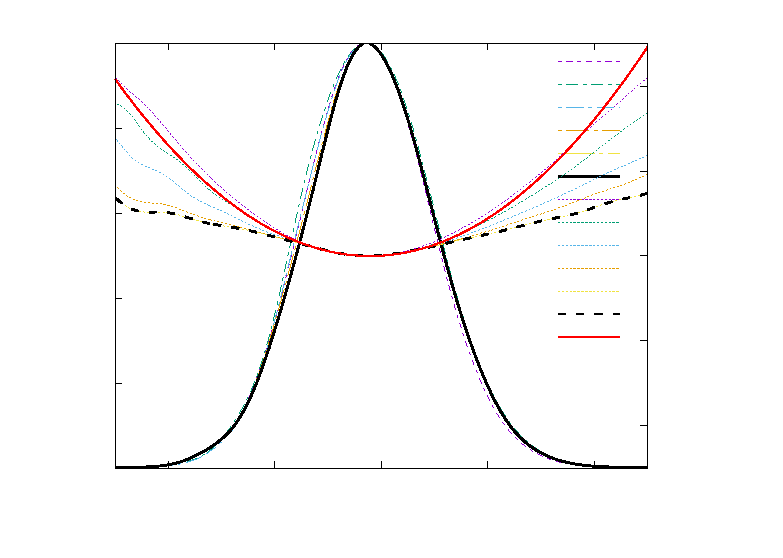
\includegraphics{spec2}}%
    \gplfronttext
  \end{picture}%
\endgroup

    \caption{Spektrale Intensität für verschiedene Einschübe $l$ mit spektraler Phase. Um die
    optimale Phase wurde ein Polynomfit zweiter Ordnung gefittet. $\Delta\lambda=27\pm1$.}
    \label{fig:spec2}
\end{figure}

\begin{figure}[]
    \begin{center}
        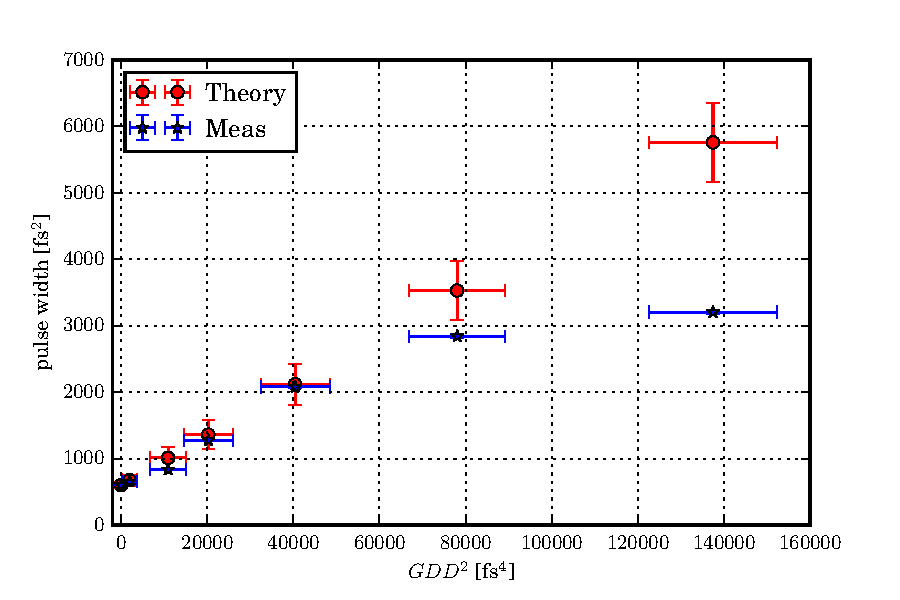
\includegraphics[width=0.7\textwidth]{Eric/prismcomp}
    \end{center}
    \caption{Theoretische und tatsächlich gemessene Pulslänge in Abhängigkeit
    von der am Prismenkompressor zum optimalen Puls hinzugefügten GDD für die
    erste Laserbandbreite. Beide werte sind quadriert worden, um einen linearen Zusammenhang zu bekommen.
    Bis auf die letzten beiden Werte, an denen der Strahl bereits vom Prisma
    abgeschnitten wurde, liegt eine sehr gute Übereinstimmung zur Theorie vor.}
    \label{fig:pckieran1}
\end{figure}
\begin{figure}[]
    \begin{center}
        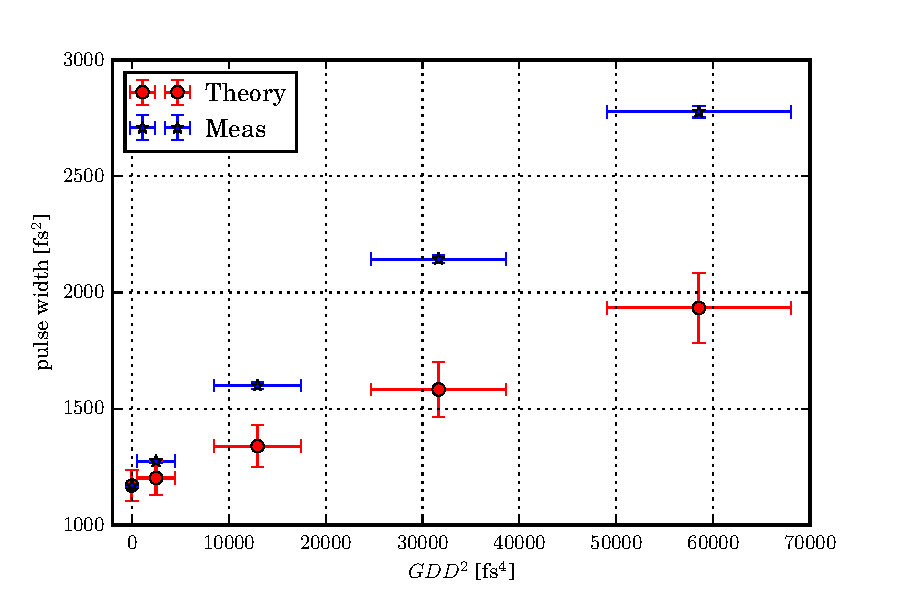
\includegraphics[width=0.7\textwidth]{Eric/prismcomp2}
    \end{center}
    \caption{Theoretische und tatsächlich gemessene Pulslänge in Abhängigkeit
    von der am Prismenkompressor zum optimalen Puls hinzugefügten GDD für die
    zweite Laserbandbreite. Beide werte sind quadriert worden, um einen linearen
    Zusammenhang zu bekommen. Da versäumt wurde, eine neue optimale
    Prismenkompressor-Position zu bestimmen, stimmen Theorie und experimentelle
    Messwerte hier nur qualitativ überein.}
    \label{fig:pckieran2}
\end{figure}
\subsection{Glasfenster}
Es wurden bei optimaler Prismenkonfiguration 5\;mm und 10\;mm BK7 Glas und
5\;mm MgF2 Glasfenster in den Strahlengang gestellt. Nach
\cref{eq:transferphase} erwartet man zwischen der GDD und der Weglänge im
Medium einen linearen Zusammenhang. Die Theoriewerte werden anhand
\cref{eq:transferphase} und \cref{eq:sellmeier} berechnet. Wieder wird mit den
kompensierten Messungen, die tatsächlich hinzugefügte GDD berechnet. Die Daten,
die in die theoretischen Werte einfließen, werden als unerheblich eingestuft.
Für die Messwerte wird wieder die Fehlerfortpflanzung mit den Werten aus dem
Prismenkompressor verwendet.
Der lineare Zusammenhang wird erfüllt, was in \cref{fig:gddkieran} zu sehen ist.
\begin{figure}[]
    \begin{center}
        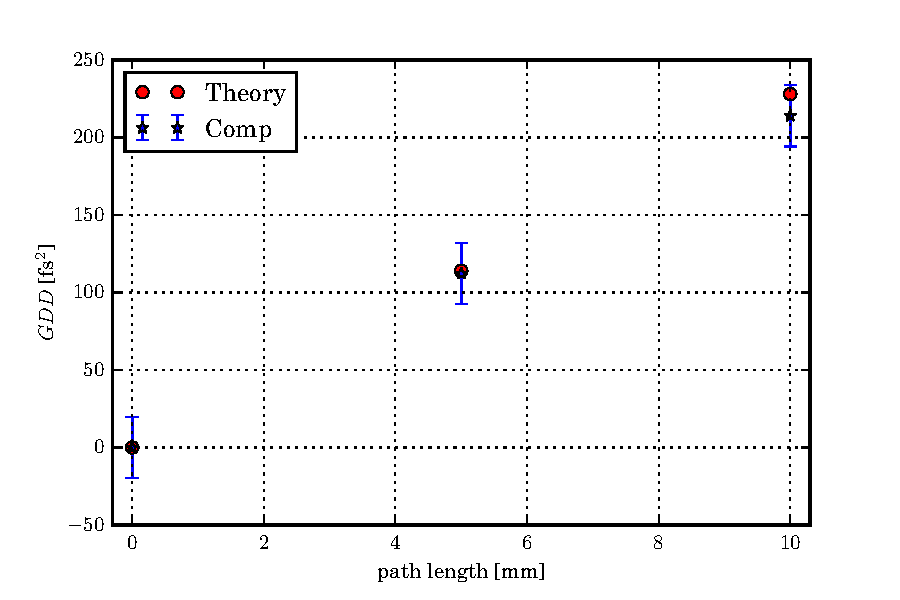
\includegraphics[width=0.5\textwidth]{Eric/glasBK7}
    \end{center}
    \caption{Betrag der GDD in Abhängigkeit der Weglänge im Glas für BK7 für
    die erste Bandbreite. In blau sind die Messwerte der kompensierten
    Messungen, in rot die theoretisch erwarteten Werte aufgetragen. Die
    Übereinstimmung ist außerordentlich gut.}
    \label{fig:gddkieran}
\end{figure}
Für das Kippen des Glases um 30$^\circ$ erwartet man außer einem räumlichen
Chirp (siehe unten) eine Verlängerung der Weglänge im Glas. Mithilfer der
Snell'schen Formeln und elementarer Trigonometrie findet man
\begin{align}
    \text{GDD}=\frac{\lambda_0^3}{4\pi
    c^2}\diff[2]{n}{\lambda}\frac{d}{\sqrt{1-\frac{\text{sin} ^2
    \alpha}{n^2}}}.
    \label{eq:tilt}
\end{align}
Bei der Messung wurde $\alpha=\pm30^\circ$ verwendet. Das Vorzeichen hat
natürlich keinen Einfluss auf die Weglänge und damit auf die GDD.
Die Resultate, inklusive derer für das MgF2 sind in Tabelle \cref{tab:glass}
zusammengefasst. In der Messung hatte das MgF2 keinerlei Auswirkungen auf die
Pulsbreite. Es wird vermutet, dass es sich hierbei um falsch abgespeicherte
Daten handelt.
Für die zweite Bandbreite ist aufgrund der fehlenden neuen Prismeneinstellung
nur eine qualitative Betrachtung sinnvoll. Die Ergebnisse sind in Tabelle
\cref{tab2} zu sehen.
\begin{table}[]
\centering
\begin{tabular}{l|r|r|r|r}
Material& $|GDD_{theo}|[\text{fs}^2]$. & $|GDD_{comp}|[\text{fs}^2]$&
$\tau_{FWHM, meas}[\text{fs}]$&$\tau_{FWHM,VChirp}[\text{fs}]$ \\
\hline
$5\, \text{mm}$ BK7&114  &$112\pm20$  &29.6 &37.5 \\
$10\, \text{mm}$ BK7&228  &$214\pm20$ &51.6 &66.7 \\
$5\, \text{mm}$ MgF2&89  & $8\pm20$ &24.4 &24.7\\
$5\, \text{mm}$ BK7 $+30^\circ$&121  &$120\pm20$&30.1 &39.1\\
$5\, \text{mm}$ BK7 $-30^\circ$& 121 &$114\pm20$ &30.6 &39.1
\end{tabular}
\caption{Zu erwartende GDD durch die optischen Elemente verglichen mit der GDD,
die beim Prismenkompressor für die Kompensierung der ersten Bandbreite eingestellt wurde. Ebenfalls eingetragen sind die gemessenen Pulslängen und jene, welche mit VCHIRP
simuliert wurden.}
\label{tab:glass}
\end{table}

\begin{table}
\centering
\begin{tabular}{l|r|r|r}
Material& $|GDD_{theo}|[\text{fs}^2]$. & $|GDD_{comp}|[\text{fs}^2]$&
$\tau_{FWHM, meas}[\text{fs}]$\\
\hline
$5\, \text{mm}$ BK7&112 &$108\pm20$  &37.2\\
$10\, \text{mm}$ BK7&223  &$200\pm20$ &49.4  
\end{tabular}
\caption{Zu erwartende GDD durch die optischen Elemente für die zweite
Bandbreite verglichen mit der GDD, die beim Prismenkompressor für die Kompensierung eingestellt wurde. Ebenfalls eingetragen sind die gemessenen Pulslängen.}
\label{tab2}
\end{table}


\subsection{Spatial Chirp und Pulse Front Tilt}
Der räumliche Chirp, welcher von der Quick-Frog Software gemessen wurde, ist
zusammen mit dem Puls Front tilt in \cref{tab:pft} aufgetragen. Für die Messung
ohne optische Elemente wurden ebenfalls beide Werte zum Vergleich eingetragen. 
Da von jedem Element höchstens zwei Datenpunkte vorhanden sind, und die ersten
per Konstruktion aufeinander fallen, wurde auf einen
Plot verzichtet. Man sieht, dass auch ohne optisches Element sowohl der PFT als
auch der räumliche Chirp nicht null sind. Deswegen ist in \cref{fig:pcpft}
beides für verschiedene Prismeneinschübe, aber ohne optisches Element
aufgetragen. Man erkennt, dass der räumliche Chirp mit steigendem
Prismeneinschub geringer wird, während der PFT wächst. Fehler wurden von der Analysesoftware nicht berechnet, aber man
kann die zeitliche Schwankungen der Messwerte größer als den Messfehler des Instrumentes
annehmen.
\begin{figure}[]
    \begin{center}
        % GNUPLOT: LaTeX picture with Postscript
\begingroup
  \makeatletter
  \providecommand\color[2][]{%
    \GenericError{(gnuplot) \space\space\space\@spaces}{%
      Package color not loaded in conjunction with
      terminal option `colourtext'%
    }{See the gnuplot documentation for explanation.%
    }{Either use 'blacktext' in gnuplot or load the package
      color.sty in LaTeX.}%
    \renewcommand\color[2][]{}%
  }%
  \providecommand\includegraphics[2][]{%
    \GenericError{(gnuplot) \space\space\space\@spaces}{%
      Package graphicx or graphics not loaded%
    }{See the gnuplot documentation for explanation.%
    }{The gnuplot epslatex terminal needs graphicx.sty or graphics.sty.}%
    \renewcommand\includegraphics[2][]{}%
  }%
  \providecommand\rotatebox[2]{#2}%
  \@ifundefined{ifGPcolor}{%
    \newif\ifGPcolor
    \GPcolortrue
  }{}%
  \@ifundefined{ifGPblacktext}{%
    \newif\ifGPblacktext
    \GPblacktexttrue
  }{}%
  % define a \g@addto@macro without @ in the name:
  \let\gplgaddtomacro\g@addto@macro
  % define empty templates for all commands taking text:
  \gdef\gplbacktext{}%
  \gdef\gplfronttext{}%
  \makeatother
  \ifGPblacktext
    % no textcolor at all
    \def\colorrgb#1{}%
    \def\colorgray#1{}%
  \else
    % gray or color?
    \ifGPcolor
      \def\colorrgb#1{\color[rgb]{#1}}%
      \def\colorgray#1{\color[gray]{#1}}%
      \expandafter\def\csname LTw\endcsname{\color{white}}%
      \expandafter\def\csname LTb\endcsname{\color{black}}%
      \expandafter\def\csname LTa\endcsname{\color{black}}%
      \expandafter\def\csname LT0\endcsname{\color[rgb]{1,0,0}}%
      \expandafter\def\csname LT1\endcsname{\color[rgb]{0,1,0}}%
      \expandafter\def\csname LT2\endcsname{\color[rgb]{0,0,1}}%
      \expandafter\def\csname LT3\endcsname{\color[rgb]{1,0,1}}%
      \expandafter\def\csname LT4\endcsname{\color[rgb]{0,1,1}}%
      \expandafter\def\csname LT5\endcsname{\color[rgb]{1,1,0}}%
      \expandafter\def\csname LT6\endcsname{\color[rgb]{0,0,0}}%
      \expandafter\def\csname LT7\endcsname{\color[rgb]{1,0.3,0}}%
      \expandafter\def\csname LT8\endcsname{\color[rgb]{0.5,0.5,0.5}}%
    \else
      % gray
      \def\colorrgb#1{\color{black}}%
      \def\colorgray#1{\color[gray]{#1}}%
      \expandafter\def\csname LTw\endcsname{\color{white}}%
      \expandafter\def\csname LTb\endcsname{\color{black}}%
      \expandafter\def\csname LTa\endcsname{\color{black}}%
      \expandafter\def\csname LT0\endcsname{\color{black}}%
      \expandafter\def\csname LT1\endcsname{\color{black}}%
      \expandafter\def\csname LT2\endcsname{\color{black}}%
      \expandafter\def\csname LT3\endcsname{\color{black}}%
      \expandafter\def\csname LT4\endcsname{\color{black}}%
      \expandafter\def\csname LT5\endcsname{\color{black}}%
      \expandafter\def\csname LT6\endcsname{\color{black}}%
      \expandafter\def\csname LT7\endcsname{\color{black}}%
      \expandafter\def\csname LT8\endcsname{\color{black}}%
    \fi
  \fi
  \setlength{\unitlength}{0.0500bp}%
  \begin{picture}(7200.00,5040.00)%
    \gplgaddtomacro\gplbacktext{%
      \csname LTb\endcsname%
      \put(814,704){\makebox(0,0)[r]{\strut{}-10}}%
      \put(814,1156){\makebox(0,0)[r]{\strut{} 0}}%
      \put(814,1609){\makebox(0,0)[r]{\strut{} 10}}%
      \put(814,2061){\makebox(0,0)[r]{\strut{} 20}}%
      \put(814,2513){\makebox(0,0)[r]{\strut{} 30}}%
      \put(814,2966){\makebox(0,0)[r]{\strut{} 40}}%
      \put(814,3418){\makebox(0,0)[r]{\strut{} 50}}%
      \put(814,3870){\makebox(0,0)[r]{\strut{} 60}}%
      \put(814,4323){\makebox(0,0)[r]{\strut{} 70}}%
      \put(814,4775){\makebox(0,0)[r]{\strut{} 80}}%
      \put(946,484){\makebox(0,0){\strut{} 0}}%
      \put(1732,484){\makebox(0,0){\strut{} 0.5}}%
      \put(2517,484){\makebox(0,0){\strut{} 1}}%
      \put(3303,484){\makebox(0,0){\strut{} 1.5}}%
      \put(4088,484){\makebox(0,0){\strut{} 2}}%
      \put(4874,484){\makebox(0,0){\strut{} 2.5}}%
      \put(5659,484){\makebox(0,0){\strut{} 3}}%
      \put(5791,704){\makebox(0,0)[l]{\strut{}-12}}%
      \put(5791,1213){\makebox(0,0)[l]{\strut{}-11.5}}%
      \put(5791,1722){\makebox(0,0)[l]{\strut{}-11}}%
      \put(5791,2231){\makebox(0,0)[l]{\strut{}-10.5}}%
      \put(5791,2740){\makebox(0,0)[l]{\strut{}-10}}%
      \put(5791,3248){\makebox(0,0)[l]{\strut{}-9.5}}%
      \put(5791,3757){\makebox(0,0)[l]{\strut{}-9}}%
      \put(5791,4266){\makebox(0,0)[l]{\strut{}-8.5}}%
      \put(5791,4775){\makebox(0,0)[l]{\strut{}-8}}%
      \put(176,2739){\rotatebox{-270}{\makebox(0,0){\strut{}Spatial chirp [$\times 10^{-5} \Delta \lambda/\Delta x$]}}}%
      \put(6692,2739){\rotatebox{-270}{\makebox(0,0){\strut{}PFT [fs/mm]}}}%
      \put(3302,154){\makebox(0,0){\strut{}Insertion $I$ [nm]}}%
    }%
    \gplgaddtomacro\gplfronttext{%
      \csname LTb\endcsname%
      \put(4672,4602){\makebox(0,0)[r]{\strut{}Spatial Chirp}}%
      \csname LTb\endcsname%
      \put(4672,4382){\makebox(0,0)[r]{\strut{}PFT}}%
    }%
    \gplbacktext
    \put(0,0){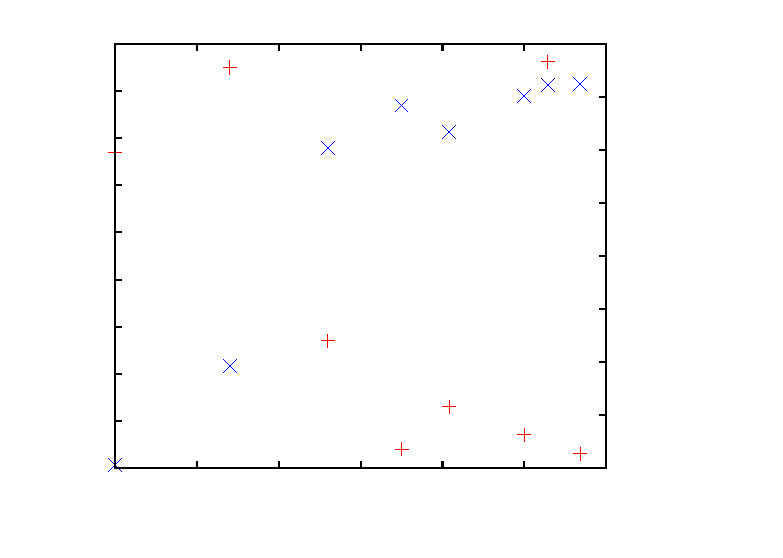
\includegraphics{pcpft}}%
    \gplfronttext
  \end{picture}%
\endgroup

    \end{center}
    \caption{Puls Front Tilt und Spatial Chirp der Prismenkompressor-Vermessung
    in Abhängigkeit der Insertion.}
    \label{fig:pcpft}
\end{figure}

\begin{table}
    \centering
    \begin{tabular}[]{|c||c|c||c|c|}
        \hline
        Objekt&\multicolumn{2}{|c||}{Spatial Chirp [$10^{-5}\Delta\lambda/\Delta x$]}&\multicolumn{2}{|c|}{Pulse front tilt [$\text{fs}/\text{mm}$]}\\\hline
         &unkompensiert&kompensiert&unkompensiert&kompensiert\\ 
        \hline
        Nur PC&$-7$&-&$-8.38$&-\\\hline
        5 mm BK7&$-30$&$-5$&$-8.52$&$-8.80$\\\hline
        10 mm BK7&$-59$&$2760$&$-8.6$&$-9.80$\\\hline
        5 mm MgF2&$-20$&$-5$&$-8.59$&$-9.01$\\\hline
        5 mm BK7 $+30^\circ$&$-28$&$0.07$&$-6.59$&$-7.86$\\\hline
        5 mm BK7 $.30^\circ$&$-31$&$-8$&$-8.44$&$-8.69$\\\hline
        BK7 Keil (wedge)&$-11$&$11$&$-15.87$&$-15.1$\\\hline
        longpass&$-90$&$-44$&$-7.06$&$-8.08$\\\hline
    \end{tabular}
    \caption{Von Quick Frog gemessener räumlicher Chirp und Puls Front Tilt,
    jeweils in optimaler (unkompensierter) Prismenkonfiguration und mit
    Kompensierung für verschiedene optische Elemente.}
    \label{tab:pft}
\end{table}
\subsection{Langpassfilter}
Für den Langpassfilter sind Intensität und Spektrum jeweils in
\cref{fig:long1,fig:long2} zusammen mit den zugehörigen Phasen sowohl in
optimaler als auch in komprensierter PC-Konfiguration aufgetragen.
Ebenfalls aufgetragen ist Intensität und Spektrum inklusive Phase der Messung
ohne Langpassfilter bei optimaler Prismenkonfiguration. Die zugehörigen
Pulsdauern und Bandbreiten sind in Tabelle \cref{tab:long} zusammengefasst.
Zum Vergleich ist für die gemessene Bandbreite der Langpass-Messung mithilfe
vom Zeit-Bandprodukt \cref{eq:bandprodeasy} die resultierende Pulsdauer eines
fourierlimitierten Pulses berechnet worden. Es ist zu erkennen, dass hier
größere Wellenlängen abgeschnitten werden, genau das Gegenteil, was man bei
einem Langpassfilter erwartet. Außerdem wird die spektrale Phase durch das
Kompensieren mit dem Prismenkompressor komplizierter und erhählt einen Knick in
Nähe des Minimums.


\begin{table}
    \centering
    \begin{tabular}[]{|c||c|c|c|c|}
        \hline
        Messung&$\tau$ [fs]&$\Delta\lambda$ [nm]&$\lambda_0$ [nm]&FWHM Zeit-Bandprodukt\\\hline
        Ohne LP (opt)&24.6&45.3&793.9&0.533\\\hline
        Langpass (opt)&56.4&34.9&784.3&0.958\\\hline
        Langpass (komp)&37.4&38.6&784.3&0.702\\\hline\hline
        Theorie &25.9&34.9&784.3&0.441\\\hline

    \end{tabular}
    \caption{Pulsdauern, Bandbreiten, Trägerwellenlängen, sowie das
    Zeit-Bandprodukt der Messungen ohne und mit Langpassfilter. Für die opt.
Langpass-Messung wurde die fourierlimitierte Pulsdauer berechnet. }
    \label{tab:long}
\end{table}


\begin{figure}[]
    \begin{center}
        % GNUPLOT: LaTeX picture with Postscript
\begingroup
  \makeatletter
  \providecommand\color[2][]{%
    \GenericError{(gnuplot) \space\space\space\@spaces}{%
      Package color not loaded in conjunction with
      terminal option `colourtext'%
    }{See the gnuplot documentation for explanation.%
    }{Either use 'blacktext' in gnuplot or load the package
      color.sty in LaTeX.}%
    \renewcommand\color[2][]{}%
  }%
  \providecommand\includegraphics[2][]{%
    \GenericError{(gnuplot) \space\space\space\@spaces}{%
      Package graphicx or graphics not loaded%
    }{See the gnuplot documentation for explanation.%
    }{The gnuplot epslatex terminal needs graphicx.sty or graphics.sty.}%
    \renewcommand\includegraphics[2][]{}%
  }%
  \providecommand\rotatebox[2]{#2}%
  \@ifundefined{ifGPcolor}{%
    \newif\ifGPcolor
    \GPcolortrue
  }{}%
  \@ifundefined{ifGPblacktext}{%
    \newif\ifGPblacktext
    \GPblacktexttrue
  }{}%
  % define a \g@addto@macro without @ in the name:
  \let\gplgaddtomacro\g@addto@macro
  % define empty templates for all commands taking text:
  \gdef\gplbacktext{}%
  \gdef\gplfronttext{}%
  \makeatother
  \ifGPblacktext
    % no textcolor at all
    \def\colorrgb#1{}%
    \def\colorgray#1{}%
  \else
    % gray or color?
    \ifGPcolor
      \def\colorrgb#1{\color[rgb]{#1}}%
      \def\colorgray#1{\color[gray]{#1}}%
      \expandafter\def\csname LTw\endcsname{\color{white}}%
      \expandafter\def\csname LTb\endcsname{\color{black}}%
      \expandafter\def\csname LTa\endcsname{\color{black}}%
      \expandafter\def\csname LT0\endcsname{\color[rgb]{1,0,0}}%
      \expandafter\def\csname LT1\endcsname{\color[rgb]{0,1,0}}%
      \expandafter\def\csname LT2\endcsname{\color[rgb]{0,0,1}}%
      \expandafter\def\csname LT3\endcsname{\color[rgb]{1,0,1}}%
      \expandafter\def\csname LT4\endcsname{\color[rgb]{0,1,1}}%
      \expandafter\def\csname LT5\endcsname{\color[rgb]{1,1,0}}%
      \expandafter\def\csname LT6\endcsname{\color[rgb]{0,0,0}}%
      \expandafter\def\csname LT7\endcsname{\color[rgb]{1,0.3,0}}%
      \expandafter\def\csname LT8\endcsname{\color[rgb]{0.5,0.5,0.5}}%
    \else
      % gray
      \def\colorrgb#1{\color{black}}%
      \def\colorgray#1{\color[gray]{#1}}%
      \expandafter\def\csname LTw\endcsname{\color{white}}%
      \expandafter\def\csname LTb\endcsname{\color{black}}%
      \expandafter\def\csname LTa\endcsname{\color{black}}%
      \expandafter\def\csname LT0\endcsname{\color{black}}%
      \expandafter\def\csname LT1\endcsname{\color{black}}%
      \expandafter\def\csname LT2\endcsname{\color{black}}%
      \expandafter\def\csname LT3\endcsname{\color{black}}%
      \expandafter\def\csname LT4\endcsname{\color{black}}%
      \expandafter\def\csname LT5\endcsname{\color{black}}%
      \expandafter\def\csname LT6\endcsname{\color{black}}%
      \expandafter\def\csname LT7\endcsname{\color{black}}%
      \expandafter\def\csname LT8\endcsname{\color{black}}%
    \fi
  \fi
  \setlength{\unitlength}{0.0500bp}%
  \begin{picture}(7200.00,5040.00)%
    \gplgaddtomacro\gplbacktext{%
      \csname LTb\endcsname%
      \put(946,704){\makebox(0,0)[r]{\strut{} 0}}%
      \put(946,1518){\makebox(0,0)[r]{\strut{} 0.2}}%
      \put(946,2332){\makebox(0,0)[r]{\strut{} 0.4}}%
      \put(946,3147){\makebox(0,0)[r]{\strut{} 0.6}}%
      \put(946,3961){\makebox(0,0)[r]{\strut{} 0.8}}%
      \put(946,4775){\makebox(0,0)[r]{\strut{} 1}}%
      \put(1078,484){\makebox(0,0){\strut{}-80}}%
      \put(1700,484){\makebox(0,0){\strut{}-60}}%
      \put(2322,484){\makebox(0,0){\strut{}-40}}%
      \put(2944,484){\makebox(0,0){\strut{}-20}}%
      \put(3567,484){\makebox(0,0){\strut{} 0}}%
      \put(4189,484){\makebox(0,0){\strut{} 20}}%
      \put(4811,484){\makebox(0,0){\strut{} 40}}%
      \put(5433,484){\makebox(0,0){\strut{} 60}}%
      \put(6055,484){\makebox(0,0){\strut{} 80}}%
      \put(6187,1111){\makebox(0,0)[l]{\strut{}-4}}%
      \put(6187,1925){\makebox(0,0)[l]{\strut{}-2}}%
      \put(6187,2740){\makebox(0,0)[l]{\strut{} 0}}%
      \put(6187,3554){\makebox(0,0)[l]{\strut{} 2}}%
      \put(6187,4368){\makebox(0,0)[l]{\strut{} 4}}%
      \put(176,2739){\rotatebox{-270}{\makebox(0,0){\strut{}Intensität $I$}}}%
      \put(6692,2739){\rotatebox{-270}{\makebox(0,0){\strut{}Phase $\Phi$ [rad]}}}%
      \put(3566,154){\makebox(0,0){\strut{}Zeit $t$ [fs]}}%
    }%
    \gplgaddtomacro\gplfronttext{%
      \csname LTb\endcsname%
      \put(5068,4602){\makebox(0,0)[r]{\strut{}$I$ LP (opt)}}%
      \csname LTb\endcsname%
      \put(5068,4382){\makebox(0,0)[r]{\strut{}$\Phi$ LP (opt)}}%
      \csname LTb\endcsname%
      \put(5068,4162){\makebox(0,0)[r]{\strut{}$I$ LP (komp)}}%
      \csname LTb\endcsname%
      \put(5068,3942){\makebox(0,0)[r]{\strut{}$\Phi$ LP (komp)}}%
      \csname LTb\endcsname%
      \put(5068,3722){\makebox(0,0)[r]{\strut{}$I$ ohne LP}}%
      \csname LTb\endcsname%
      \put(5068,3502){\makebox(0,0)[r]{\strut{}$\Phi$ ohne LP}}%
    }%
    \gplbacktext
    \put(0,0){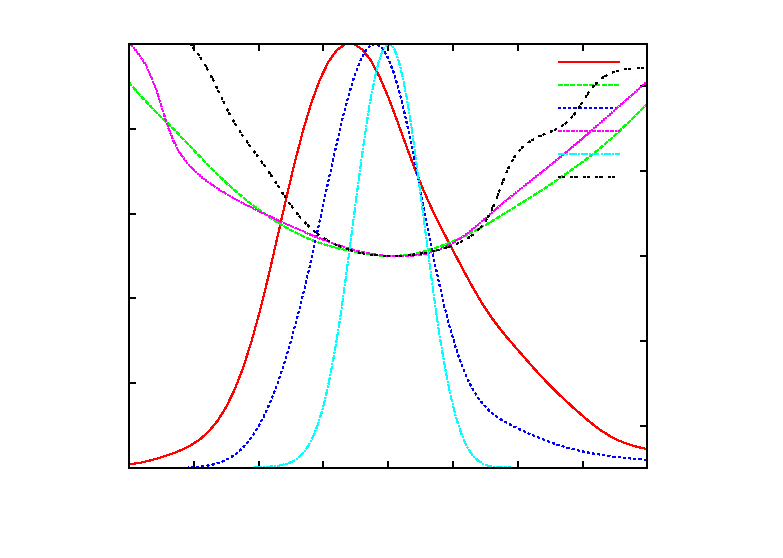
\includegraphics{longpass}}%
    \gplfronttext
  \end{picture}%
\endgroup

    \end{center}
    \caption{Intensität bei optimaler Prismenkonfiguration (opt) ohne
    Langpassfilter und bei
    eingesetztem Langpassfilter unkompensiert und kompensiert.}
    \label{fig:long1}
\end{figure}

\begin{figure}[]
    \begin{center}
        % GNUPLOT: LaTeX picture with Postscript
\begingroup
  \makeatletter
  \providecommand\color[2][]{%
    \GenericError{(gnuplot) \space\space\space\@spaces}{%
      Package color not loaded in conjunction with
      terminal option `colourtext'%
    }{See the gnuplot documentation for explanation.%
    }{Either use 'blacktext' in gnuplot or load the package
      color.sty in LaTeX.}%
    \renewcommand\color[2][]{}%
  }%
  \providecommand\includegraphics[2][]{%
    \GenericError{(gnuplot) \space\space\space\@spaces}{%
      Package graphicx or graphics not loaded%
    }{See the gnuplot documentation for explanation.%
    }{The gnuplot epslatex terminal needs graphicx.sty or graphics.sty.}%
    \renewcommand\includegraphics[2][]{}%
  }%
  \providecommand\rotatebox[2]{#2}%
  \@ifundefined{ifGPcolor}{%
    \newif\ifGPcolor
    \GPcolortrue
  }{}%
  \@ifundefined{ifGPblacktext}{%
    \newif\ifGPblacktext
    \GPblacktexttrue
  }{}%
  % define a \g@addto@macro without @ in the name:
  \let\gplgaddtomacro\g@addto@macro
  % define empty templates for all commands taking text:
  \gdef\gplbacktext{}%
  \gdef\gplfronttext{}%
  \makeatother
  \ifGPblacktext
    % no textcolor at all
    \def\colorrgb#1{}%
    \def\colorgray#1{}%
  \else
    % gray or color?
    \ifGPcolor
      \def\colorrgb#1{\color[rgb]{#1}}%
      \def\colorgray#1{\color[gray]{#1}}%
      \expandafter\def\csname LTw\endcsname{\color{white}}%
      \expandafter\def\csname LTb\endcsname{\color{black}}%
      \expandafter\def\csname LTa\endcsname{\color{black}}%
      \expandafter\def\csname LT0\endcsname{\color[rgb]{1,0,0}}%
      \expandafter\def\csname LT1\endcsname{\color[rgb]{0,1,0}}%
      \expandafter\def\csname LT2\endcsname{\color[rgb]{0,0,1}}%
      \expandafter\def\csname LT3\endcsname{\color[rgb]{1,0,1}}%
      \expandafter\def\csname LT4\endcsname{\color[rgb]{0,1,1}}%
      \expandafter\def\csname LT5\endcsname{\color[rgb]{1,1,0}}%
      \expandafter\def\csname LT6\endcsname{\color[rgb]{0,0,0}}%
      \expandafter\def\csname LT7\endcsname{\color[rgb]{1,0.3,0}}%
      \expandafter\def\csname LT8\endcsname{\color[rgb]{0.5,0.5,0.5}}%
    \else
      % gray
      \def\colorrgb#1{\color{black}}%
      \def\colorgray#1{\color[gray]{#1}}%
      \expandafter\def\csname LTw\endcsname{\color{white}}%
      \expandafter\def\csname LTb\endcsname{\color{black}}%
      \expandafter\def\csname LTa\endcsname{\color{black}}%
      \expandafter\def\csname LT0\endcsname{\color{black}}%
      \expandafter\def\csname LT1\endcsname{\color{black}}%
      \expandafter\def\csname LT2\endcsname{\color{black}}%
      \expandafter\def\csname LT3\endcsname{\color{black}}%
      \expandafter\def\csname LT4\endcsname{\color{black}}%
      \expandafter\def\csname LT5\endcsname{\color{black}}%
      \expandafter\def\csname LT6\endcsname{\color{black}}%
      \expandafter\def\csname LT7\endcsname{\color{black}}%
      \expandafter\def\csname LT8\endcsname{\color{black}}%
    \fi
  \fi
  \setlength{\unitlength}{0.0500bp}%
  \begin{picture}(7200.00,5040.00)%
    \gplgaddtomacro\gplbacktext{%
      \csname LTb\endcsname%
      \put(946,704){\makebox(0,0)[r]{\strut{} 0}}%
      \put(946,1518){\makebox(0,0)[r]{\strut{} 0.2}}%
      \put(946,2332){\makebox(0,0)[r]{\strut{} 0.4}}%
      \put(946,3147){\makebox(0,0)[r]{\strut{} 0.6}}%
      \put(946,3961){\makebox(0,0)[r]{\strut{} 0.8}}%
      \put(946,4775){\makebox(0,0)[r]{\strut{} 1}}%
      \put(1078,484){\makebox(0,0){\strut{} 740}}%
      \put(1983,484){\makebox(0,0){\strut{} 760}}%
      \put(2888,484){\makebox(0,0){\strut{} 780}}%
      \put(3793,484){\makebox(0,0){\strut{} 800}}%
      \put(4698,484){\makebox(0,0){\strut{} 820}}%
      \put(5603,484){\makebox(0,0){\strut{} 840}}%
      \put(6187,704){\makebox(0,0)[l]{\strut{}-3}}%
      \put(6187,1383){\makebox(0,0)[l]{\strut{}-2}}%
      \put(6187,2061){\makebox(0,0)[l]{\strut{}-1}}%
      \put(6187,2740){\makebox(0,0)[l]{\strut{} 0}}%
      \put(6187,3418){\makebox(0,0)[l]{\strut{} 1}}%
      \put(6187,4097){\makebox(0,0)[l]{\strut{} 2}}%
      \put(6187,4775){\makebox(0,0)[l]{\strut{} 3}}%
      \put(176,2739){\rotatebox{-270}{\makebox(0,0){\strut{}Spektrale Intensität $S$}}}%
      \put(6692,2739){\rotatebox{-270}{\makebox(0,0){\strut{}Spektrale Phase $\varphi$ [rad]}}}%
      \put(3566,154){\makebox(0,0){\strut{}Wellenlänge $\lambda$ [nm]}}%
    }%
    \gplgaddtomacro\gplfronttext{%
      \csname LTb\endcsname%
      \put(5068,4602){\makebox(0,0)[r]{\strut{}$I$ LP (opt)}}%
      \csname LTb\endcsname%
      \put(5068,4382){\makebox(0,0)[r]{\strut{}$\varphi$ LP (opt)}}%
      \csname LTb\endcsname%
      \put(5068,4162){\makebox(0,0)[r]{\strut{}$I$ LP (komp)}}%
      \csname LTb\endcsname%
      \put(5068,3942){\makebox(0,0)[r]{\strut{}$\varphi$ LP (komp)}}%
      \csname LTb\endcsname%
      \put(5068,3722){\makebox(0,0)[r]{\strut{}$I$ ohne LP}}%
      \csname LTb\endcsname%
      \put(5068,3502){\makebox(0,0)[r]{\strut{}$\varphi$ ohne LP}}%
    }%
    \gplbacktext
    \put(0,0){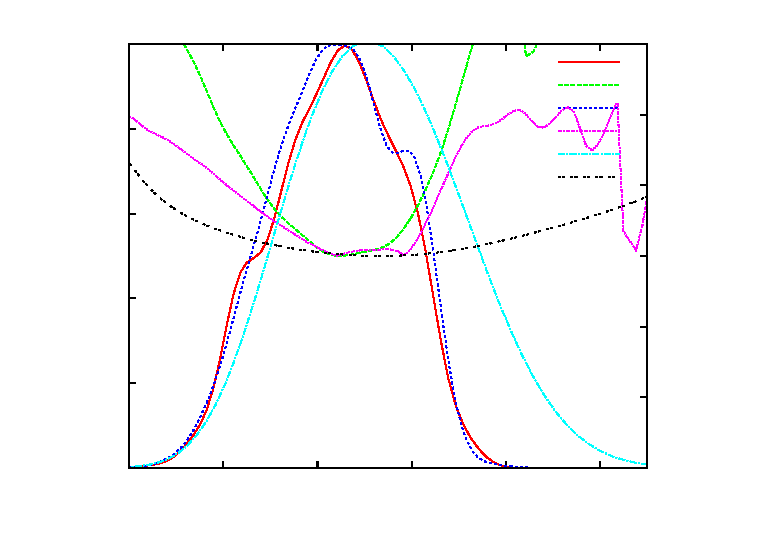
\includegraphics{longpass2}}%
    \gplfronttext
  \end{picture}%
\endgroup

    \end{center}
    \caption{Spektrum bei optimaler Prismenkonfiguration (opt) ohne
    Langpassfilter und mit eingesetztem Langpassfilter, unkompensiert und
    kompensiert.}
    \label{fig:long2}
\end{figure}

\subsection{Dielektrische Spiegel}
Die Messung für Pfad 2 mit den drei dielektrischen Spiegeln ergab ein sehr
verzerrtes FROG-Trace (\cref{fig:diel}). Als vergleich ist der Trace der optimalen
Prismenkompressor-Messung in \cref{fig:opttrace} zu sehen. Aufgrund dieser
Verzerrung und da der FROG-error sehr groß ist, ist keine sinnvolle
Rekonstruktion der Pulsform möglich. Ebenso ist aus dem Spektrum keine
sinnvolle Information zu entnehmen, außer dass hier erhebliche Verzerrungen
auftreten. Die Pulsform wird von den dielektrischen Spiegeln regelrecht
zerstört. Auch eine Kompensierung mit dem Prismenkompressor war unmöglich: Die
Pulsdauer war absolut unberührt von dem Einschub des zweiten Prismas.

\begin{figure}[]
    \centering
    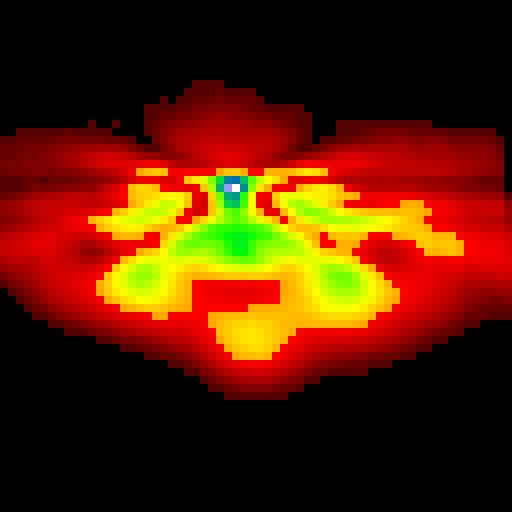
\includegraphics[width=0.3\textwidth]{diel.jpg}
    \caption{Experimenteller FROG trace für die Messung mit dielektrischen
    Spiegeln. Der Trace ist sehr verzerrt, wodurch keine sinnvolle
Rekonstruktion der Pulsform möglich ist. }
    \label{fig:diel}
\end{figure}
\begin{figure}[]
    \centering
    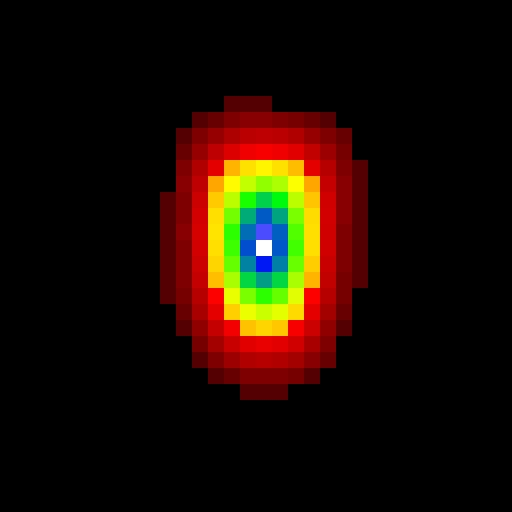
\includegraphics[width=0.3\textwidth]{opttrace.jpg}
    \caption{Experimenteller FROG trace der optimalen Prismenkompressormessung.}
    \label{fig:opttrace}
\end{figure}

\subsection{Rechteckiges Spiegelpaar}
Für die Rechteckspiegel mit jeweils 5 Reflektionen zeichnet sich ein ähnliches
Bild, wie für die dielektrischen Spiegel ab. Der FROG-Trace ist verzerrt
und der FROG error ist groß ebenso sind der rekonstruierte FROG trace stark
unterschiedlich vom experimentellen. Die Ergebnisse sind in \cref{fig:chirpspiegel1}
für die unkompensierte, sowie in \cref{fig:chirpspiegel2} für die kompensierte
Messung zu sehen. Allerdings sind die Verzerrungen hier nicht so stark wie
zuvor. Die Pulsintensität, sowie das Spektrum mit Phase sind in
\cref{fig:chirptemp,fig:chirpspec} zu sehen. Man erkennt eine deutliche
Phasenfluktuation, sowie eine große Pulsbreite bei den kompensierten
Prismenkompressoreinstellungen. Die Messungen in optimaler Einstellung sind
stattdessen mit Ausnahme von einigen Einschneidungen in der Intensität nahezu
Gaußförmig, wenn auch mit deutlich größerer Pulsdauer im Vergleich zu den 
metallischen Spiegeln. Es ist anzunehmen, dass es sich hier um gechirpte
Spiegel handelt, die eine große negative GDD liefern. Dieser Effekt wird
verstärkt durch die mehreren Reflektionen. Dies würde erklären, wieso die
Pulsform bei den ``kompensierten'' Messungen verzerrter ist: Der
Prismen-Kompressor addiert noch mehr negativen GDD hinzu.


\begin{figure}[]
    \centering
    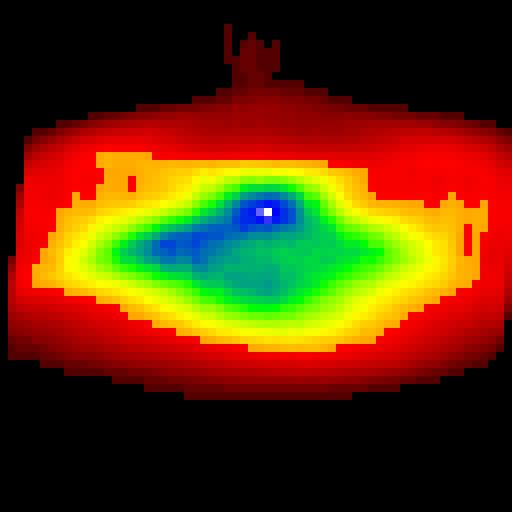
\includegraphics[width=0.3\textwidth]{chirpsp1.jpg}
    \caption{Experimenteller FROG trace des Spiegelpaares}
    \label{fig:chirpspiegel1}
\end{figure}
\begin{figure}[]
    \centering
    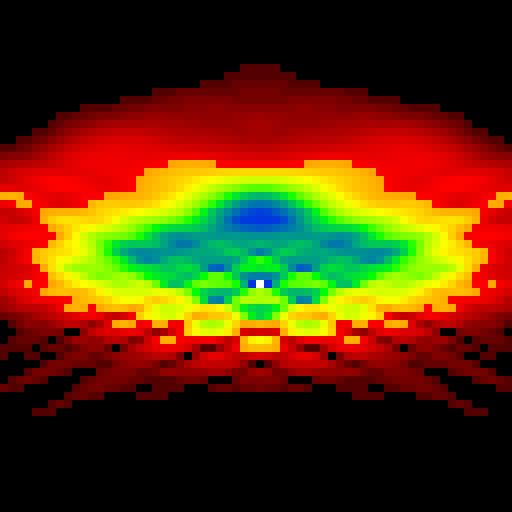
\includegraphics[width=0.3\textwidth]{chirpsp2.jpg}
    \caption{Rekonstruierter FROG trace des Spiegelpaares}
    \label{fig:chirpspiegel2}
\end{figure}
\begin{figure}[]
    \centering
    % GNUPLOT: LaTeX picture with Postscript
\begingroup
  \makeatletter
  \providecommand\color[2][]{%
    \GenericError{(gnuplot) \space\space\space\@spaces}{%
      Package color not loaded in conjunction with
      terminal option `colourtext'%
    }{See the gnuplot documentation for explanation.%
    }{Either use 'blacktext' in gnuplot or load the package
      color.sty in LaTeX.}%
    \renewcommand\color[2][]{}%
  }%
  \providecommand\includegraphics[2][]{%
    \GenericError{(gnuplot) \space\space\space\@spaces}{%
      Package graphicx or graphics not loaded%
    }{See the gnuplot documentation for explanation.%
    }{The gnuplot epslatex terminal needs graphicx.sty or graphics.sty.}%
    \renewcommand\includegraphics[2][]{}%
  }%
  \providecommand\rotatebox[2]{#2}%
  \@ifundefined{ifGPcolor}{%
    \newif\ifGPcolor
    \GPcolortrue
  }{}%
  \@ifundefined{ifGPblacktext}{%
    \newif\ifGPblacktext
    \GPblacktexttrue
  }{}%
  % define a \g@addto@macro without @ in the name:
  \let\gplgaddtomacro\g@addto@macro
  % define empty templates for all commands taking text:
  \gdef\gplbacktext{}%
  \gdef\gplfronttext{}%
  \makeatother
  \ifGPblacktext
    % no textcolor at all
    \def\colorrgb#1{}%
    \def\colorgray#1{}%
  \else
    % gray or color?
    \ifGPcolor
      \def\colorrgb#1{\color[rgb]{#1}}%
      \def\colorgray#1{\color[gray]{#1}}%
      \expandafter\def\csname LTw\endcsname{\color{white}}%
      \expandafter\def\csname LTb\endcsname{\color{black}}%
      \expandafter\def\csname LTa\endcsname{\color{black}}%
      \expandafter\def\csname LT0\endcsname{\color[rgb]{1,0,0}}%
      \expandafter\def\csname LT1\endcsname{\color[rgb]{0,1,0}}%
      \expandafter\def\csname LT2\endcsname{\color[rgb]{0,0,1}}%
      \expandafter\def\csname LT3\endcsname{\color[rgb]{1,0,1}}%
      \expandafter\def\csname LT4\endcsname{\color[rgb]{0,1,1}}%
      \expandafter\def\csname LT5\endcsname{\color[rgb]{1,1,0}}%
      \expandafter\def\csname LT6\endcsname{\color[rgb]{0,0,0}}%
      \expandafter\def\csname LT7\endcsname{\color[rgb]{1,0.3,0}}%
      \expandafter\def\csname LT8\endcsname{\color[rgb]{0.5,0.5,0.5}}%
    \else
      % gray
      \def\colorrgb#1{\color{black}}%
      \def\colorgray#1{\color[gray]{#1}}%
      \expandafter\def\csname LTw\endcsname{\color{white}}%
      \expandafter\def\csname LTb\endcsname{\color{black}}%
      \expandafter\def\csname LTa\endcsname{\color{black}}%
      \expandafter\def\csname LT0\endcsname{\color{black}}%
      \expandafter\def\csname LT1\endcsname{\color{black}}%
      \expandafter\def\csname LT2\endcsname{\color{black}}%
      \expandafter\def\csname LT3\endcsname{\color{black}}%
      \expandafter\def\csname LT4\endcsname{\color{black}}%
      \expandafter\def\csname LT5\endcsname{\color{black}}%
      \expandafter\def\csname LT6\endcsname{\color{black}}%
      \expandafter\def\csname LT7\endcsname{\color{black}}%
      \expandafter\def\csname LT8\endcsname{\color{black}}%
    \fi
  \fi
    \setlength{\unitlength}{0.0500bp}%
    \ifx\gptboxheight\undefined%
      \newlength{\gptboxheight}%
      \newlength{\gptboxwidth}%
      \newsavebox{\gptboxtext}%
    \fi%
    \setlength{\fboxrule}{0.5pt}%
    \setlength{\fboxsep}{1pt}%
\begin{picture}(7200.00,5040.00)%
    \gplgaddtomacro\gplbacktext{%
      \csname LTb\endcsname%
      \put(814,704){\makebox(0,0)[r]{\strut{}$0$}}%
      \put(814,1518){\makebox(0,0)[r]{\strut{}$0.2$}}%
      \put(814,2332){\makebox(0,0)[r]{\strut{}$0.4$}}%
      \put(814,3147){\makebox(0,0)[r]{\strut{}$0.6$}}%
      \put(814,3961){\makebox(0,0)[r]{\strut{}$0.8$}}%
      \put(814,4775){\makebox(0,0)[r]{\strut{}$1$}}%
      \put(946,484){\makebox(0,0){\strut{}$-250$}}%
      \put(1457,484){\makebox(0,0){\strut{}$-200$}}%
      \put(1968,484){\makebox(0,0){\strut{}$-150$}}%
      \put(2479,484){\makebox(0,0){\strut{}$-100$}}%
      \put(2990,484){\makebox(0,0){\strut{}$-50$}}%
      \put(3501,484){\makebox(0,0){\strut{}$0$}}%
      \put(4011,484){\makebox(0,0){\strut{}$50$}}%
      \put(4522,484){\makebox(0,0){\strut{}$100$}}%
      \put(5033,484){\makebox(0,0){\strut{}$150$}}%
      \put(5544,484){\makebox(0,0){\strut{}$200$}}%
      \put(6055,484){\makebox(0,0){\strut{}$250$}}%
      \put(6187,1111){\makebox(0,0)[l]{\strut{}$-4$}}%
      \put(6187,1925){\makebox(0,0)[l]{\strut{}$-2$}}%
      \put(6187,2740){\makebox(0,0)[l]{\strut{}$0$}}%
      \put(6187,3554){\makebox(0,0)[l]{\strut{}$2$}}%
      \put(6187,4368){\makebox(0,0)[l]{\strut{}$4$}}%
    }%
    \gplgaddtomacro\gplfronttext{%
      \csname LTb\endcsname%
      \put(176,2739){\rotatebox{-270}{\makebox(0,0){\strut{}Intensität $I$}}}%
      \put(6692,2739){\rotatebox{-270}{\makebox(0,0){\strut{}Phase $\Phi$ [rad]}}}%
      \put(3500,154){\makebox(0,0){\strut{}Zeit $t$ [fs]}}%
      \csname LTb\endcsname%
      \put(5068,4602){\makebox(0,0)[r]{\strut{}$I$ (opt)}}%
      \csname LTb\endcsname%
      \put(5068,4382){\makebox(0,0)[r]{\strut{}$\Phi$ (opt)}}%
      \csname LTb\endcsname%
      \put(5068,4162){\makebox(0,0)[r]{\strut{}$I$ (komp)}}%
      \csname LTb\endcsname%
      \put(5068,3942){\makebox(0,0)[r]{\strut{}$\Phi$ (komp)}}%
    }%
    \gplbacktext
    \put(0,0){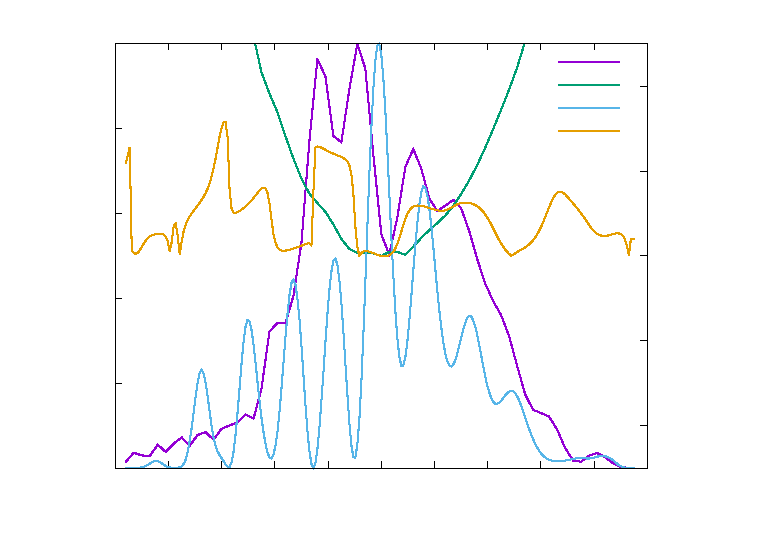
\includegraphics{chirptemp}}%
    \gplfronttext
  \end{picture}%
\endgroup

    \caption{Experimenteller FROG trace des Spiegelpaares}
    \label{fig:chirptemp}
\end{figure}
\begin{figure}[]
    \centering
    % GNUPLOT: LaTeX picture with Postscript
\begingroup
  \makeatletter
  \providecommand\color[2][]{%
    \GenericError{(gnuplot) \space\space\space\@spaces}{%
      Package color not loaded in conjunction with
      terminal option `colourtext'%
    }{See the gnuplot documentation for explanation.%
    }{Either use 'blacktext' in gnuplot or load the package
      color.sty in LaTeX.}%
    \renewcommand\color[2][]{}%
  }%
  \providecommand\includegraphics[2][]{%
    \GenericError{(gnuplot) \space\space\space\@spaces}{%
      Package graphicx or graphics not loaded%
    }{See the gnuplot documentation for explanation.%
    }{The gnuplot epslatex terminal needs graphicx.sty or graphics.sty.}%
    \renewcommand\includegraphics[2][]{}%
  }%
  \providecommand\rotatebox[2]{#2}%
  \@ifundefined{ifGPcolor}{%
    \newif\ifGPcolor
    \GPcolortrue
  }{}%
  \@ifundefined{ifGPblacktext}{%
    \newif\ifGPblacktext
    \GPblacktexttrue
  }{}%
  % define a \g@addto@macro without @ in the name:
  \let\gplgaddtomacro\g@addto@macro
  % define empty templates for all commands taking text:
  \gdef\gplbacktext{}%
  \gdef\gplfronttext{}%
  \makeatother
  \ifGPblacktext
    % no textcolor at all
    \def\colorrgb#1{}%
    \def\colorgray#1{}%
  \else
    % gray or color?
    \ifGPcolor
      \def\colorrgb#1{\color[rgb]{#1}}%
      \def\colorgray#1{\color[gray]{#1}}%
      \expandafter\def\csname LTw\endcsname{\color{white}}%
      \expandafter\def\csname LTb\endcsname{\color{black}}%
      \expandafter\def\csname LTa\endcsname{\color{black}}%
      \expandafter\def\csname LT0\endcsname{\color[rgb]{1,0,0}}%
      \expandafter\def\csname LT1\endcsname{\color[rgb]{0,1,0}}%
      \expandafter\def\csname LT2\endcsname{\color[rgb]{0,0,1}}%
      \expandafter\def\csname LT3\endcsname{\color[rgb]{1,0,1}}%
      \expandafter\def\csname LT4\endcsname{\color[rgb]{0,1,1}}%
      \expandafter\def\csname LT5\endcsname{\color[rgb]{1,1,0}}%
      \expandafter\def\csname LT6\endcsname{\color[rgb]{0,0,0}}%
      \expandafter\def\csname LT7\endcsname{\color[rgb]{1,0.3,0}}%
      \expandafter\def\csname LT8\endcsname{\color[rgb]{0.5,0.5,0.5}}%
    \else
      % gray
      \def\colorrgb#1{\color{black}}%
      \def\colorgray#1{\color[gray]{#1}}%
      \expandafter\def\csname LTw\endcsname{\color{white}}%
      \expandafter\def\csname LTb\endcsname{\color{black}}%
      \expandafter\def\csname LTa\endcsname{\color{black}}%
      \expandafter\def\csname LT0\endcsname{\color{black}}%
      \expandafter\def\csname LT1\endcsname{\color{black}}%
      \expandafter\def\csname LT2\endcsname{\color{black}}%
      \expandafter\def\csname LT3\endcsname{\color{black}}%
      \expandafter\def\csname LT4\endcsname{\color{black}}%
      \expandafter\def\csname LT5\endcsname{\color{black}}%
      \expandafter\def\csname LT6\endcsname{\color{black}}%
      \expandafter\def\csname LT7\endcsname{\color{black}}%
      \expandafter\def\csname LT8\endcsname{\color{black}}%
    \fi
  \fi
    \setlength{\unitlength}{0.0500bp}%
    \ifx\gptboxheight\undefined%
      \newlength{\gptboxheight}%
      \newlength{\gptboxwidth}%
      \newsavebox{\gptboxtext}%
    \fi%
    \setlength{\fboxrule}{0.5pt}%
    \setlength{\fboxsep}{1pt}%
\begin{picture}(7200.00,5040.00)%
    \gplgaddtomacro\gplbacktext{%
      \csname LTb\endcsname%
      \put(814,704){\makebox(0,0)[r]{\strut{}$0$}}%
      \put(814,1518){\makebox(0,0)[r]{\strut{}$0.2$}}%
      \put(814,2332){\makebox(0,0)[r]{\strut{}$0.4$}}%
      \put(814,3147){\makebox(0,0)[r]{\strut{}$0.6$}}%
      \put(814,3961){\makebox(0,0)[r]{\strut{}$0.8$}}%
      \put(814,4775){\makebox(0,0)[r]{\strut{}$1$}}%
      \put(946,484){\makebox(0,0){\strut{}$740$}}%
      \put(1875,484){\makebox(0,0){\strut{}$760$}}%
      \put(2804,484){\makebox(0,0){\strut{}$780$}}%
      \put(3733,484){\makebox(0,0){\strut{}$800$}}%
      \put(4662,484){\makebox(0,0){\strut{}$820$}}%
      \put(5591,484){\makebox(0,0){\strut{}$840$}}%
      \put(6187,704){\makebox(0,0)[l]{\strut{}$-3$}}%
      \put(6187,1383){\makebox(0,0)[l]{\strut{}$-2$}}%
      \put(6187,2061){\makebox(0,0)[l]{\strut{}$-1$}}%
      \put(6187,2740){\makebox(0,0)[l]{\strut{}$0$}}%
      \put(6187,3418){\makebox(0,0)[l]{\strut{}$1$}}%
      \put(6187,4097){\makebox(0,0)[l]{\strut{}$2$}}%
      \put(6187,4775){\makebox(0,0)[l]{\strut{}$3$}}%
    }%
    \gplgaddtomacro\gplfronttext{%
      \csname LTb\endcsname%
      \put(176,2739){\rotatebox{-270}{\makebox(0,0){\strut{}Spektrale Intensität $S$}}}%
      \put(6692,2739){\rotatebox{-270}{\makebox(0,0){\strut{}Spektrale Phase $\varphi$ [rad]}}}%
      \put(3500,154){\makebox(0,0){\strut{}Wellenlänge $\lambda$ [nm]}}%
      \csname LTb\endcsname%
      \put(5068,4602){\makebox(0,0)[r]{\strut{}$S$ (opt)}}%
      \csname LTb\endcsname%
      \put(5068,4382){\makebox(0,0)[r]{\strut{}$\varphi$ (opt)}}%
      \csname LTb\endcsname%
      \put(5068,4162){\makebox(0,0)[r]{\strut{}$S$ (komp)}}%
      \csname LTb\endcsname%
      \put(5068,3942){\makebox(0,0)[r]{\strut{}$\varphi$ (komp)}}%
    }%
    \gplbacktext
    \put(0,0){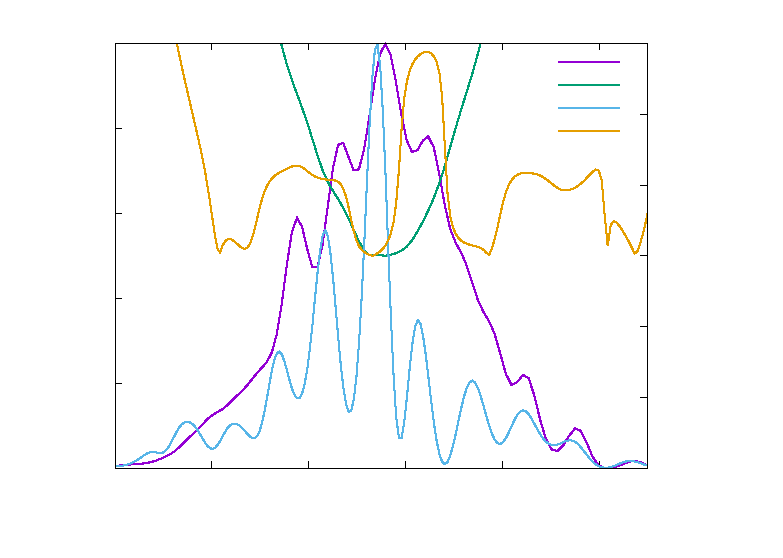
\includegraphics{chirpspec}}%
    \gplfronttext
  \end{picture}%
\endgroup

    \caption{Rekonstruierter FROG trace des Spiegelpaares}
    \label{fig:chirpspec}
\end{figure}

\newpage
\section{Diskussion}
\subsection{Prismenkompressor}
Zunächst ist aus \cref{fig:temp1,fig:temp2} zu sehen, dass die Pulslänge für
die optimale Prismenkompressor-Einstellung tatsächlich minimal ist. Desweiteren
ist bei der ersten Laserbandbreiten-Einstellung die optimale Phase weniger
gekrümmt als alle anderen: Ihre zweite Ordnung ist gering. Dies sagt aus, dass
der lineare Chirp in dieser Einstellung tatsächlich minimiert wurde. Dennoch
konnte nicht erreicht werden, dass der Chirp komplett verschwindet. Dies ist
jedoch zu erwarten, da die Einstellung des Prismenkompressors beim Suchen des
Pulsminimas im Experiment relativ ungenau war, dar es eine breite Einstellung
des Prismas gab, bei der die Pulslänge von Quick Frog als nahezu konstant
angezeigt wurde. Weiterhin erkennt man, dass der Puls in der Zeit minimal
verschiebt wurde (ca. 0.002\;fs). Dies sagt aus, dass die spektrale Phase
annäherend keinen linearen Anteil hat, was die Näherung während der Umrechnung
der GDD in fs$^{-1}$ rechtfertigt. Bei der zweiten Lasereinstellung ist dies
nicht mehr der Fall: Der Puls ist um einige Femtosekunden zeitlich verschoben.
Demnach ist der Messwert für die GDD der zweiten Bandbreite ungenauer. Dies ist
auch qualitativ aus \cref{fig:spec2} zu sehen, da die Phase hier einen Knick im
Minimum hat. Bei Betrachtung des Spektrums der ersten Bandbreite fällt auf,
dass für verschiedene Einschübe das Spektrum verschoben wird. Dies bedeutet,
dass die zeitliche Phase einen nicht verschwindenden linearen Anteil (GD)
aufweist. Man erkennt, dass sich die Bandbreite minimal ändert, was bedeutet,
dass der größte Einfluss auf die Pulslänge tatsächlich die GDD ist, wie
erwartet. Auch hier ist deutlich, dass die spektrale Phase in optimaler
Einstellung minimal ist, demnach ist der Puls nahezu ungechirpt.
Für die zweite Bandbreite hätte man eine neue Prismenkompressor-Position finden
müssen, bei der die Pulslänge minimiert wird. Der hier gefundene optimale Wert
für die erste Bandbreite liefert zwar ebenfalls für die zweite Bandbreite eine
minimale Pulslänge, allerdings hätte man für noch größere Einschübe
wahrscheinlich eine noch kürzere Pulslänge erhalten können.\\
Da der Laser nahezu ungechirpt aus dem PC austritt, wenn dieser in optimaler
Position ist, ist das Vorgehen für die Vermessung des PC's gerechtfertigt. Die
Bestimmung des Einschubes durch die Position, ab der der Laser am Prisma
vorbeifliegt ist jedoch recht ungenau, was auch die großen Messungenauigkeiten
und die Fehlerintervalle in den Theoriewerten in
\cref{fig:pckieran1,fig:pckieran2} hervorruft. Für die erste Bandbreite ist die
Übereinstimmung der Theorie- und Messwerte hervorragend. Lediglich als der
Laser angefangen hat, am Prisma vorbeizuschießen wird hier eine signifikante
Abweichung erreicht. Für die zweite Bandbreite ist die Steigung der sich
bildenden geraden offensichtlich falsch im Vergleich zur Theorie. Hier ist als
Ursache die fehlerhafte Prismenkonfiguration zu nennen.
\subsection{Glasfenster}
Die Messungen für die Glasfenster sind generell ins sehr guter Übereinstimmung
mit den theoretischen Werten. So ist bei allen Gläsern außer dem MgF2 der
Theoriewert innerhalb des Fehlerintervalls der Messwerte. Diese wurden aber
auch durch die ungenaue Messung der Prismenkompressor-Größen relativ groß
gewählt. Die relativen
Abweichungen sind nur ca. $5\%$. Man kann deswegen der Pulskomprimierung des
Prismenkompressors vertrauen. Einzig und allein die Messung für das MgF2 Glas
ergibt völlig falsche Ergebnisse. Wie bereits im Auswertungs-Abschnitt
geschildert, muss es sich hier um falsche Daten handeln. Entweder wurden die
richtigen Daten aus versehen überschrieben, oder Der Laser hat das Glas nicht
getroffen, was aber sehr unwahrscheinlich ist. Die gemessenen Pulslängen sind
ebenfalls in einigermaßen guter Übereinstimmung zu den mit VChirp simulierten
Werten. Hier findet man einen relativen Fehler von ca. 25\%. Eine Erklärung
hierfür ist, dass bei VChirp ein völlig ungechirpter Puls Gaußpuls benutzt
wurde. Es ist anzumerken, dass die Fehler vom Quick-Frog Programm nicht
geliefert wurden. Man hat während des Versuchs jedoch eine zeitliche Schwankung
der Messwerte erkannt. Diese Fehler wurden bei der Auswertung linear
interpoliert und sind in die Unsicherheitsintervalle bereits eingeflossen. Es ist zu sehen, dass die Simulationsergebnisse eine größere Pulslänge
vorhersagen. Dies ist konsistent mit der Annahme, dass nach
\cref{eq:pulsverbreiterung} ein Puls mit kürzerer Pulslänge mehr
Pulsverbreiterung durch Dispersion erlebt.
Die Werte für die zweite Laser-Bandbreite sind ebenfalls in guter
Übereinstimmung mit der Theorie, obwohl keine neue PC Position bestimmt wurde.
Der relative Fehler beträgt hier ca 10\%. 
\subsection{Spatial Chirp und Pulse Front Tilt}
Bei dem schiefen Glas erwartet man als zusätzlichen Effekt einen räumlichen
Chirp. Es ist jedoch zu sehen, dass das nicht schiefe Glas einen ungefähr
gleichen räumlichen Chirp aufweist. Den mit Abstand größten räumlichen Chirp
weist der Langpassfilter auf, obwohl man hier theoretisch keinen Einfluss
erwartet. Eine mögliche Fehlerquelle ist ein ungenaues, bzw schiefes Einbauen
der optischen Elemente. Vergleicht man die kompensierten Werte, so ergibt sich
der allgemeine Trend, dass der Spatial Chirp mit mehr Kompensation geringer
wird. Mehr Kompensation bedeutet hier weniger Einschub des Prismas. Deswegen
ist dieser Trend bei der Vermessung des Prismenkompressors in \cref{fig:pcpft}
bestätigt. Die Ursache ist womöglich ein ungenau ausgerichteter
Prismenkompressor, da bei optimaler Einstellung kein räumlicher Chirp auftreten
sollte. Ein offensichtlicher Ausreißer ist das 10\;mm BK7 Glas mit einem
Wert von 2070$\times10^{-5}\Delta\lambda/\Delta x$. Es ist wahrscheinlich, dass
diese Anomalie von einem Fehlerhaften Messen, zum Beispiel einer Über- oder
Unterbelichtung kommt.\\
Für den PFT erkennt man zwar, dass der Prismenkompressor bei mehr Einschub
einen größeren PFT liefert, dennoch ist der PFT bei dem Keil ungefähr zweimal
so groß wie bei allen anderen Messungen, entspricht also den Erwartungen, dass
der Keil zu einem zusätzlichen PFT führt.
\subsection{Langpassfilter}
Zunächst ist anzumerken, dass es sich hier höchstwahrscheinlich um einen
Shortpass-Filter handelt. Wahrscheinlich wurden die beiden Filter aus versehen
vertauscht. Im Experiment konnte durch den ``Short-Pass'' benannten Filter,
keine Intensität durchkommen. Deswegen könnte es auch sein, dass die
Abschneide-Wellenlänge eine Falsche ist. Es ist aus \cref{tab:long} zu
erkennen, dass die Pulslängen nach Durchlaufen des Filters wesentlich länger
sind, als von einem nahezu ungechirpten Puls erwartet, was man anhand des
größeren Zeit-Bandproduktes erkennen kann. Auch in der Grafik des Spektrums
(\cref{fig:long2} ist zu sehen, dass die spektrale Phase einen Knick nahe des
Minimums hat. Interessant ist hier, dass eine Kompensation mit dem
Prismenkompressor die Verzerrung der spektralen Phase nur verstärkt, insgesamt
aber dennoch der Puls kürzer wird. Dies liegt daran, dass der unkompensierte
Puls einen relativ langen Schwanz auf der positiven Zeitachse besitzt, während
der komprimierte Puls dies nicht aufweist. Dies könnte zum Beispiel ein Effekt
von einer Dispersion höherer Ordnung sein.
\subsection{Dielektrische Spiegel}
Für die Dielektrischen Spiegel waren offensichtlich keine Sinnvollen Pulslängen
bestimmbar. Dies ergibt Sinn, wenn diese nicht für Ultrakurzlaser angefertigt
sind. Dielektrische Spiegel absorbieren unterschiedliche Wellenlängen durch
ihre verschiedenen Schichtdicken unterschiedlich stark und dies führt zu einer
Verzögerung die stark abhängig von der Wellenlänge ist. Deswegen kann die Phase
des einlaufenden Pulses durch diese Interferenz stark verzerrt werden. 
Es ist also wichtig, vor dem Experiment zu überprüfen, ob die dielektrischen
Spiegel für Ultrakurzzeit-Experimente geeignet sind. Metallische Spiegel haben
diese Gefahr nicht, allerdings liefern sie auch schlechtere Reflektivitäten als
korrekt präparierte dielektrische Spiegel.
\subsection{Gechirpte Spiegel}
Wie bereits in der Auswertung erwähnt, handelt es sich wahrscheinlich um
gechirpte Spiegelpaare. Dies wird daraus gefolgert, dass die Pulsform bei
kompensierter Messung verzerrter war, als vorher. Dies wäre dadurch zu
erklären, dass die Spiegel bereits eine hohe negative GDD hervorrufen, was
durch die negative GDD des Prismenkompressors nur noch weiter verstärkt wird.
Hier hätte man versuchen können, in die andere Richtung zu drehen, um bei dem
Prismenkompressor positive GDD zu erzeugen. Es ist jedoch fraglich, ob man
genug positive GDD erzeugen könnte. 
Gechirpte Spiegel sind demnach wie der Prismenkompressor eine Möglichkeit die
positive GDD von optischen Bauteilen zu kompensieren. Da der Prismenkompressor
in unserer Einstellung nur negative GDD liefert, sind die Verzerrungen also zu
erwarten.

\section{Kritik am Versuchsaufbau und dem Handbuch}
Bei diesem Versuch handelt es sich um einen relativ neuen Versuch. Deswegen ist
mit ein paar Problemen zu rechnen. Der Versuchsaufbau hat kaum Probleme
bereitet. Es war gut, dass man fast alles noch einmal justieren sollte, um ein
Gefühl für die Justage zu bekommen, bevor die eigentlichen Messungen angefangen
haben. Der größte Kritikpunkt fällt hier auf die verwendete Software Quick
Frog: Es war teilweise nicht zu erkennen, wann das Programm bereit war, neue
Daten zu sammeln, was zum Beispiel zu Ausreißern wie beim Spatial Chirp oder
beim MgF2 Glas führen kann. Das größte Problem war allerdings, wie das Programm
Daten gespeichert hat. So war es sehr mühsam, durch alle Ordner zu gehen und
die relevanten Daten zu sammeln, besonders Weil viele Daten ausschließlich über
einen Screenshot einsehbar waren.
Das Handbuch war gut verständlich und man wusste eigentlich immer, was beim
Versuch zu machen war. Allerdings hätte ich mich über eine etwas konkretere
Aufgabenstellung für die Datenauswertung gefreut. Die Aufgaben sind
(wahrscheinlich gewollt) sehr offen gestellt. Es heißt nur ``Werten Sie die
Daten aus''. Dies zusammen damit, dass keine relevanten Formeln gegeben waren
und auch die Literatur nicht eingegrenzt wurde, machte die Literaturrecherche
für diesen Versuch sehr aufwendig. Natürlich hat man Formeln gefunden, war sich
aber nie sicher, ob sie brauchbar sind, oder nicht, bzw ob man überhaupt eine
Auswertung solcher Art durchführen sollte. Besonders für jemanden, der vorher
keine Erfahrung mit nichtlinearer Optik gemacht hat, war es also eine große
Herausforderung. Der zeitliche Rahmen für diesen Versuch wurde für 1.5 Credits
somit bei weitem gesprengt. Es wäre also sinnvoll, genauere Arbeitsaufträge zu
geben, wie ``Führen Sie einen Phasenfit um das Spektrum aus'', oder ``benutzen
Sie folgende Formel, um \ldots'' und außerdem die Literatur etwas
einzuschränken, vielleicht die wirklich relevanten Kapitel ausgedruckt parat zu
haben. Dies würde zumindest ein Gefühl von
Sicherheit gewähren, dass man nicht völlig auf dem falschen Pfad ist, ein
Gefühl was ich leider für einen Großteil der Zeit hatte.
Dennoch hat man, besonders im Labor, viel über das praktische Arbeiten mit
Laserquellen und die Justage von optischen Aufbauten gelernt, was meine
Erwartungen an diesen Versuch erfüllt hat.



\bibliography{literatur}

\end{document}

